\documentclass[a4paper,11pt]{kth-mag}
\let\ifpdf\relax
\usepackage[T1]{fontenc}
\usepackage{textcomp}
\usepackage{lmodern}
%\usepackage[latin1]{inputenc}
\usepackage[swedish,english]{babel}
\usepackage{modifications}
\usepackage{amsmath}
\usepackage{ifpdf}
\usepackage[breaklinks=true]{hyperref}
\usepackage{breakcites}
\usepackage{pdfpages}
\usepackage{booktabs}

\newcommand{\textunderscript}[1]{$_{\text{#1}}$}
\usepackage[utf8]{inputenc}
%\usepackage{cite}
%\usepackage{biblatex}
%\addbibresource{references.bib}
%\newenvironment{italicquotes}
%{\begin{quote}\itshape}
%{\end{quote}}

%% Graphic packages
\usepackage{graphicx}
\usepackage{tikz}
\usepackage{tikz-3dplot}
\usetikzlibrary{positioning}
%\usepackage{circuitikz}
\usetikzlibrary{calc,patterns,decorations.pathmorphing,decorations.markings}
\usepackage{subcaption}
\usepackage{tikz-cd}
\usetikzlibrary{decorations.text}

\tikzset{
    %Define standard arrow tip
    >=stealth',
    %Define style for boxes
    punkt/.style={
           rectangle,
           rounded corners,
           draw=black, very thick,
           text width=6.5em,
           minimum height=2em,
           text centered},
    % Define arrow style
    pil/.style={
           ->,
           thick,
           shorten <=2pt,
           shorten >=2pt,}
}




%\usepackage{appendix} 
\title{The Black Box}
\subtitle{Control and design of reaction wheel inverted pendulum}
\foreigntitle{Reglering och design av inverterad pendel med hjälp av svänghjul}
\author{Mikael Sjöstedt \\ Alexander Ramm}
\date{May 2015}
\blurb{ Bachelor's Thesis in Mechatronics \vspace{1em} \\
\begin{tabular}{ll} 
Supervisor: Daniel Frede &  \\
Examiner: Martin Edin Grimheden \\ 
Approved: TBA 2015-month-day
\end{tabular} }
\trita{TRITA MMK 2015:18 MDAB071}


\begin{document}


\includepdf[pages={1}]{kth-cover.pdf}
\clearpage

\frontmatter
\pagestyle{plain}
%\removepagenumbers
\pagenumbering{roman}
\maketitle
\selectlanguage{english}
\begin{abstract}
\addcontentsline{toc}{chapter}{Abstract}
Some robots can do remarkable things. Balancing something unstable is one of them. This paper covers the design of such a robot and evaluates how the sensor is affected by its position and in turn the robots ability to balance. A robot with a reaction wheel to maintain balance was built and the sensor data was investigated.

From the result one could see that the sensor placement was of importance. The best placement was the one closest to the center of the cube, far away from the reaction wheel.
 
\end{abstract}
\cleardoublepage
\begin{foreignabstract}{swedish}
\addcontentsline{toc}{chapter}{Sammanfattning}
En del robotar kan utföra förbluffande manövrar. Att balansera något instabilt är en av dem. Den här rapporten täcker konstruktionen av en sådan robot och undersöker hur sensorn påverkas av sin position och i sin tur hur balansförmågan påverkas av sensorn. En robot som använde ett svänghjul som hjälp för att balansera byggdes och sensordatan undersöktes.

Från resultatet visade att sensorplaceringen var viktig. Den bästa placeringen var den närmast den robotens centrum.
\\


%Examensarbetet skrivs på engelska och har alltid både en svensk och en engelsk sammanfattningssida. Denna skrivmall, som inte har ``bookmarks'' eller några avancerade ``features'', definierar layouten för ett examensarbete i Maskinteknik (MF123X) eller Industriell ekonomi (MF105X).
%I detta kapitel sammanfattas examensarbetet. Sammanfattningens omfattning är högst en sida. Sammanfattningen åtföljs av en blank sida. Den föregående titelsidan, som lämpligen också innehåller en illustrativ bild, följs också av en blank sida. Alla kapitel börjar längst upp på en högersida, dvs på ett udda sidonummer.
\end{foreignabstract}
\clearpage
\chapter*{Preface}
\addcontentsline{toc}{chapter}{Preface}
We would like to thank Daniel Frede, our supervisor, for his continuous support, always ready with a well filled beer glass and pinpointing our faults with \textit{German precision}.

Staffan Qvarnström and Tomas Östberg for their mechanical and practical expertise and counselling.

We would also like to thank our fellow student colleagues David Tennander \& Viktor Gjurovski, who has been carrying out an equivalent project, for rewarding discussions and ideas.

Furthermore Filip Stenbeck and Aron Nygren for their inspiration and enthusiasm. And definitely all the student assistants who have helped us throughout the course.


\begin{flushright}Alexander Ramm \\Mikael Sjöstedt \\ KTH, may, 2015 \end{flushright}
 

%\clearpage


\cleardoublepage
\addcontentsline{toc}{chapter}{Contents}
\printindex
\tableofcontents*

\cleardoublepage
\chapter*{Nomenclature}
\addcontentsline{toc}{chapter}{Nomenclature}
\section*{Symbols}
\noindent{}\begin{tabular}{@{}p{2.5cm}l}
\textbf{Symbol} 	& \textbf{Description} \vspace{.5em} \\
$\mathcal{L}$			& Lagrangian \\
$\theta$		& Cube angle (Rad)\\
$\phi$		& Flywheel angle (Rad) \\
$q$			& Lagrange operator \\
$E_k	$		& Kinetic energy (J)\\
$E_p$		& Potential Energy (J)\\
$I_c$		& Inertia of the cube (Kg $\cdot$ m\textsuperscript{2})\\
$I_f$		& Inertia of the flywheel (Kg $\cdot$ m\textsuperscript{2})\\
$M\textsubscript{tot}$		& Total mass of the cube (Kg)\\
$M_f$		& Mass of the flywheel (Kg)\\
$i$			& Current (Amp)\\
$K_t$		& Motor torque constant (Nm / Amp)\\
E\textunderscript{emf} 	& Induced voltage (V)\\
K\textunderscript{emf} 	& Motor voltage constant (V $\cdot$ s/Rad)\\
U			& Voltage across motor poles (V)\\
$R_m	$		& Motor internal resistance (Ohm)\\
$\eta_m$		& Motor efficiency\\	
$\eta_g$		& Gear efficiency \\
$\Gamma$		& Gear ratio\\
$z$			& Measurement noise \\
$w$			& Process noise \\

\end{tabular}
\clearpage

\section*{Abbreviations}
\noindent{}\begin{tabular}{@{}p{2.5cm}l}
\textbf{Abbreviation} 	& \textbf{Description} \vspace{.5em} \\
CAD			& Computer Aided Design \\
CAE			& Computer Aided Engineering\\
DC			& Direct Current \\
DOF			& Degrees of freedom\\
dps			& Degrees per second\\
IC			& Integrated circuit\\
$I^2C$		& Inter-Integrated circuit\\
IDE 			& Integrated Development Interface \\
LSB			& Least significant bit \\
MCU			& Microcontroller\\
MEMS			& Microelectromechanical Systems \\
PLM			& Product Lifecycle Management\\
PWM			& Pulse With Modulation\\
RMS			& Root Mean Square\\
RPM			& Revolutions per minute\\
UAV			& Unmanned Aerial Vehicle\\
USB			& Universal Serial Bus
\end{tabular}
\cleardoublepage

\mainmatter
\pagestyle{newchap}


\chapter{Introduction}

\epigraph{\textit{“If there are two or more ways to do something, and one of those ways can result in a catastrophe, then someone will do it.”}}{Edward A. Murphy Jr.}

This chapter describes the background, purpose and scope of this project conducted at the mechatronics department at the Royal Institute of Technology, KTH, Sweden. The work was carried out during the spring 2015.

\section{Background}
A reaction wheel is a wheel that is accelerated to apply torque. The most widespread use of reaction wheels is in human made satellites. The  reaction wheels, usually three of them in the case of satellites, are used to change the attitude of the satellite by applying torque in a favourable manner. This is imperative to direct solar panels towards the sun or pointing antennas to assure maximum performance and connectivity to the satellite. Satellites are quite uncommon (there are just over thousand satellites currently in orbit), and their technology can at times seem alien. But reaction wheels should not be alienated, they can be used in many contexts and this paper will cover one of them.  

Balancing a one \textit{degree of freedom} (DOF) inverted pendulum type structure using a reaction wheel is no new concept, and became more accessible with the introduction of cheap microcontrollers.
The use of automated control has been growing at a rapid pace the last decades and is being implemented
more and more in consumer related products.  

This growth has made automated control together with sensors available more now than ever. It can be seen in the every-day life in product lines such as mobile phones, gaming controllers, cars and UAVs such as quadrocopters.

One of the most basic systems that requires some control to become stable is the inverted pendulum. 
Although it is simple to define, its control is not. A lot of work has been done on the topic
but there are still a limited amount of knowledge available to the public. 

The method to achieve balance of a pendulum using reaction wheels is even more narrow. 
In recent years prototypes of land based structures using reaction wheels have been a hot topic and some of these robots are truly remarkable. 
It would be a great achievement for the authors to contribute knowledge about how such a device could be built and evaluate some of
the capabilities and restrictions of such a machine.


\section{Purpose}
The goal of the project was to build a structure with one degree of freedom that can maintain balance using a reaction wheel and examine the behaviours of the system. A concept idea of the robot can be seen in Figure \ref{Figure: concept idea}
\begin{figure}[!htb] 
\centering
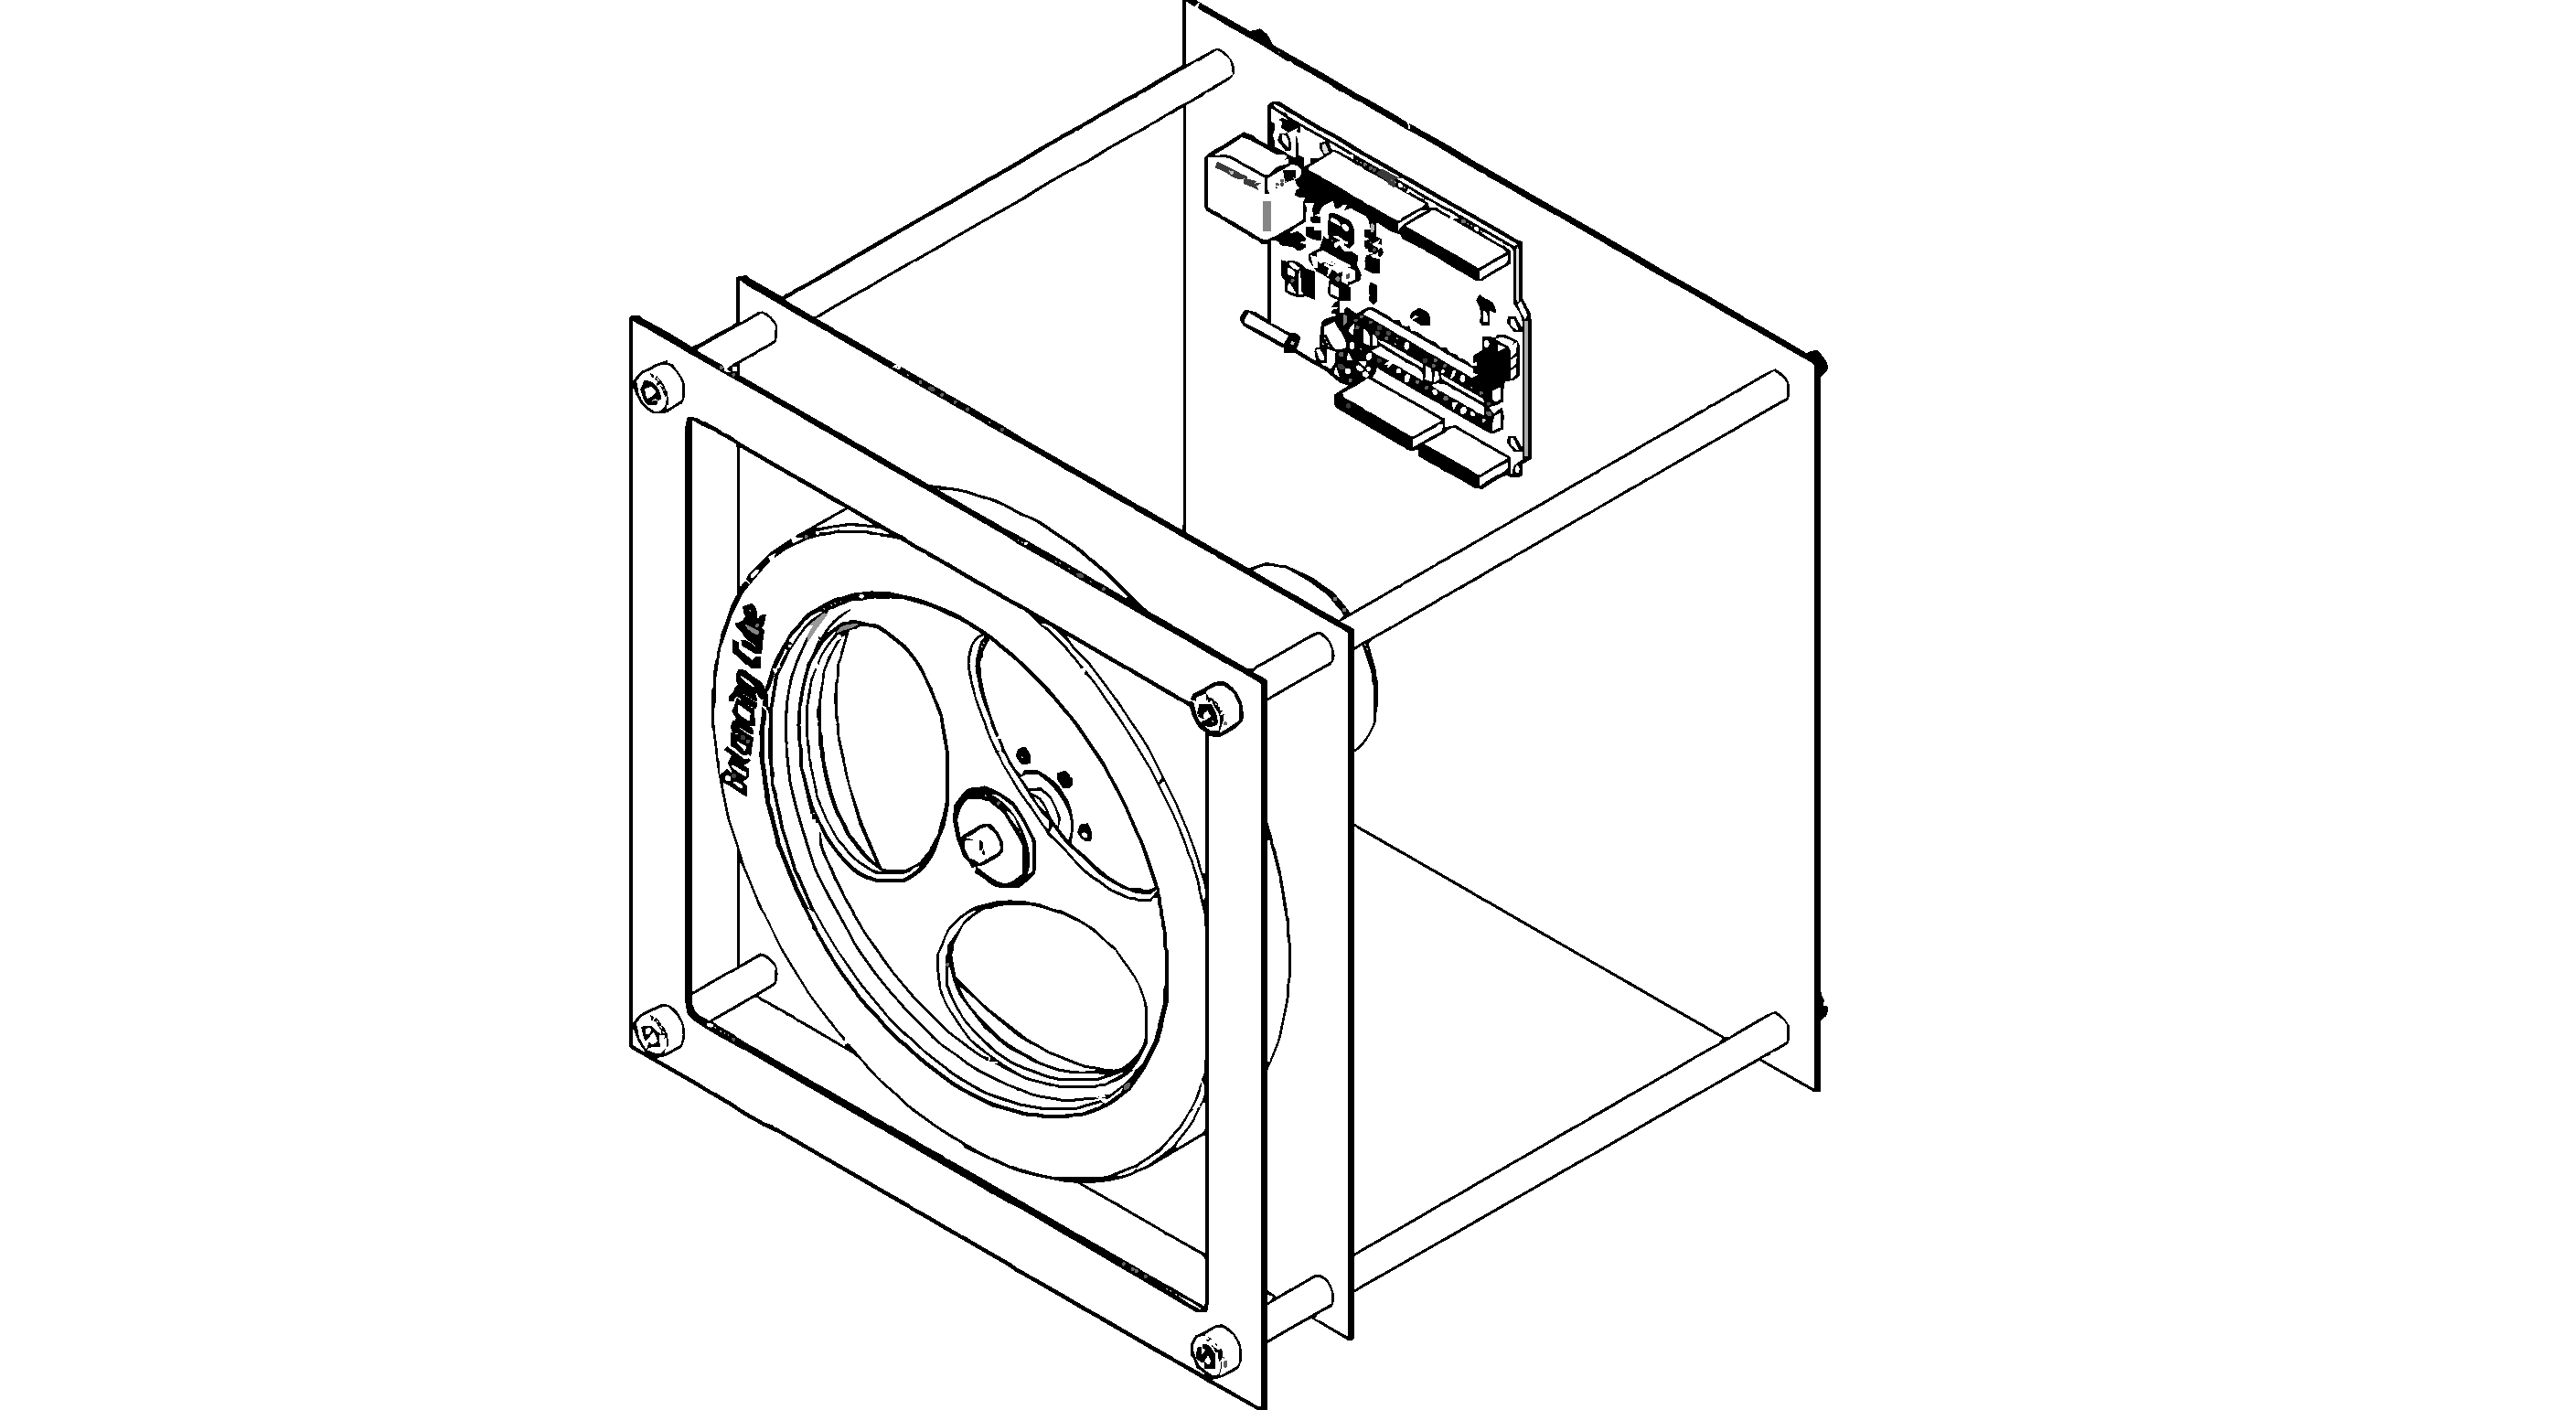
\includegraphics[width = \textwidth]{concept.pdf}
\caption{Concept design}
\label{Figure: concept idea}
\end{figure}

The dynamics is mostly effected by the control system, which is responsible for accelerating the motor and thus the reaction wheel in the  correct angular direction, to maintain balance. The parameters in the control system effects response time, overshoot and sinusoidal settling time.
This project will hopefully contribute to some development within the open-source community.
All results are available online, open source on GitHub \cite{Github}.
As a thesis in mechatronics, this paper can be divided into two parts. One engineering part whose focus is to implement knowledge in mechanics, electronics and control theory to result in a functioning robot. A research part whose topic was to investigate how the system was effected by sensor placement. This could be concentrated to a question 

\begin{quote}
\textit{
What sensor position is least inflicted by noise, when the cube is stationary?
} \\

\textit{How much does the best and worst position effect the system performance when balancing?
}
\end{quote}


The sensors used for this project is an \textit{Inertial Measurement Unit} (IMU) which can be placed arbitrarily. Certain positions might have an advantage in terms of how usable the raw data is. The IMU is a sensitive devise and disturbances such as high current and fast oscillations in its vicinity might effect the data, which is to be investigated. 

\section{Scope}
The sensor which position were to be examined was an IMU. Only a few key positions of the sensor was examined.

The effects that were looked at was the ones related to the control system. Only data from the IMU axes used in the specific control system were examined, the placement effect on other axes was not taken into consideration.

All control model dynamics was done non-discretely.

\section{Method} \label{sec: method}
At first, data from the IMU was collected at different positions during a stationary state where the frame was rigidly mounted. The motor was accelerated with a sinusoidal current to simulate the same conditions as during a balancing state. The IMU was then moved to a position closer to the motor with the hypothesis that the motor induce an electrical field that effects the measurement unit.
Six recordings were made for each placement and the variance was calculated thereafter.



\begin{figure}
\centering
\begin{subfigure}{.48\textwidth}
  \centering
  \includegraphics[trim=0.3cm 0.1cm 0.8cm 0.2cm, clip=true, width=\textwidth]{framsidaIMUpunkter.jpg}
  \caption{IMU placement, front}
  \label{Fig: IMU placement front}
\end{subfigure}
\begin{subfigure}{.48\textwidth}
  \centering
  \includegraphics[trim=0.6cm 0.15cm 0.5cm 0.2cm, clip=true, width=\textwidth]{baksidaIMUpunkter.jpg}
  \caption{IMU placement, back}
  \label{Fig: IMU placement back}
\end{subfigure}
\caption{IMU placements}
\label{Fig: IMU placement}
\end{figure}

Five different positions were examined. They can be seen in Figure \ref{Fig: IMU placement}. Six measurements were taken for every position. The expected value and standard deviation for the particular position was calculated.

Then a comparative between the position with the least and most standard deviation were done
to try how the system performance was effected. The cube was placed at rest close to the balance point with the help of a support. The support was removed with the control system enabled. The time taken for the cube to fall on its side was measured.


\chapter{Theory} \label{chapter: theory}
\epigraph{\textit{"Nothing is as easy as it looks."}}{Murphy's law}
This chapter cover some of the theory that is required if one would want to build a similar robot. It is assumed that the reader has some understanding of Newtonian mechanics, signal analysis and control theory. Basic understanding of DC motor operation is also an advantage.

The first part is about the inertial reference unit that covers issues of sensor characteristics and why they are important to the system as a whole and the research question in particular.

There is a part that discuss Kalman filter theory, a filter required for retrieving high quality data from the IMU. The filter interprets noisy data from the sensor and digitally filters the signal to a more trustworthy output. 

The last part covers the theory of the mechanical system behaviour that is used to develop the regulator. The equations are responsible for the actual balance part and thus important. 

\section{Inertial Measurement Unit} \label{section:IMU}
\subsection{Background}
The data collected for calculating the angle of the cube is gathered from an IMU, a unit that uses both an accelerometer and a gyroscope to track the orientation and position. An IMU is often rated for several degrees of freedom, a unit specified as 6-DOF usually uses three orthogonal accelerometers and gyroscopes. These measure linear acceleration and angular velocity respectively. There are also units that are rated for additional degrees of freedom and usually include features such as magnetometer or barometer sensors.   
To understand the fundamentals of an inertial navigation system a Cartesian coordinate system is defined in Figure \ref{Figure: cartesian}

\begin{figure}[!hbt] 
\centering
\tdplotsetmaincoords{60}{110}
%
\pgfmathsetmacro{\rvec}{.8}
\pgfmathsetmacro{\thetavec}{30}
\pgfmathsetmacro{\phivec}{60}
%

\begin{tikzpicture}[scale=6,tdplot_main_coords]
    \coordinate (O) at (0,0,0);
    \draw[thick,->] (0,0,0) -- (1,0,0) node[anchor=north east]{$x$};
    \draw[thick,->] (0,0,0) -- (0,1,0) node[anchor=north west]{$y$};
\draw[thick,->] (0,0,0) -- (0,0,1) node[anchor=south]{$z$};
	\node at (0.5,0,0) (x) {};

\tdplotdrawarc[->,color=black]{(0,0,0.6)}{0.1}{0}{340}{anchor=south west,color=black}{yaw}
%We move to the z-x axis
\tdplotsetthetaplanecoords{0}

\tdplotdrawarc[tdplot_rotated_coords,->,color=black]{(0,0,0.6)}{0.1}{110}{450}{anchor=south west,color=black}{pitch}
\tdplotsetthetaplanecoords{-90}

\tdplotdrawarc[tdplot_rotated_coords,->,color=black]{(0,0,0.6)}{0.1}{120}{460}{anchor=south west,color=black}{roll}

\end{tikzpicture}
\caption{Cartesian coordinate system}
\label{Figure: cartesian}
\end{figure}
 
The accelerometer is used to measure the acceleration along the lines of $x,y,z$ axes while the gyroscope measures the angular rate around these axes.
 
The inertial navigation system used in this project is a small \textit{microelectro-mechanical system} (MEMS). A micromechanical sensor is a very small unit that make use of its mechanical properties to sense alteration in the environment \cite{ref:accelerometero}. The advantages of these small units are low production costs, small size, low power consumption and good accuracy. But all these advantages comes at a price, which is signal noise \cite{IMUintro}.
\subsection{Accelerometer} \label{sec: accelerometer}
Accelerometers are used to measure linear acceleration. Or rather, it measure forces due to acceleration. These forces can be divided into two groups
\begin{itemize}
\item Static forces, such as gravity
\item Dynamic forces, due to movement
\end{itemize}
The force is then converted into acceleration, this is done by measuring the change of capacitance when a spring mass system is moving.

The typical accelerometer consists of a movable mass that is attached via a mechanical spring or suspension system to a frame that is used as reference. 
The capacitance is usually measured between a conductive plate and the known mass, seen in figure \ref{Fig: Accelerometer}. The capacitance is thereafter used to determine the displacement of the mass and then calculate the force applied to it with the known spring mass system.

\begin{figure} [!hbt]
\centering
\begin{tikzpicture} [every node/.style={draw,outer sep=0pt,thick},]

\tikzstyle{spring}=[thick,decorate,decoration={zigzag,pre length=0.3cm,post length=0.3cm,segment length=6}]
\tikzstyle{damper}=[thick,decoration={markings,  
  mark connection node=dmp,
  mark=at position 0.5 with 
  {
    \node (dmp) [thick,inner sep=0pt,transform shape,rotate=-90,minimum width=15pt,minimum height=3pt,draw=none] {};
    \draw [thick] ($(dmp.north east)+(2pt,0)$) -- (dmp.south east) -- (dmp.south west) -- ($(dmp.north west)+(2pt,0)$);
    \draw [thick] ($(dmp.north)+(0,-5pt)$) -- ($(dmp.north)+(0,5pt)$);
  }
}, decorate]
\tikzstyle{ground}=[fill,pattern=north east lines,draw=none,minimum width=0.75cm,minimum height=0.3cm]



\begin{scope}[]
\node (M) [minimum width=1cm, minimum height=2.5cm] {$m$};

\node (ground) [ground,anchor=north,yshift=-0.25cm,minimum width=1.5cm] at (M.south) {};
\draw (ground.north east) -- (ground.north west);
\draw [thick] (M.south west) ++ (0.2cm,-0.125cm) circle (0.125cm)  (M.south east) ++ (-0.2cm,-0.125cm) circle (0.125cm);

\node (wall) [ground, rotate=-90, minimum width=3cm,yshift=-3cm] {};
\draw (wall.north east) -- (wall.north west);

\draw [spring] (wall.170) -- ($(M.north west)!(wall.170)!(M.south west)$);
\draw [damper] (wall.10) -- ($(M.north west)!(wall.10)!(M.south west)$);

\node (arrow) [draw=none, above right = -0.5cm and 0 cm of M, label={[xshift=0.7cm, yshift=0cm] $\Delta$ C}] {};
\draw [<->,thick] (arrow) ++ (0.2cm,0) -- +(1cm,0);

\end{scope}

%\draw[step=1cm,gray,very thin] (-2,-2) grid (6,6);
\draw [thick] (2.2,-1.3) -- (2.2,1.3);
%\node (wall2) [thick,rotate = 90, minimum width = 3cm, xshift = 0cm, yshift = -2.5cm] {};
%\draw [thick] (wall2.east) -- (wall2.east);
 


\end{tikzpicture}
\caption{Accelerometer capacitance }
\label{Fig: Accelerometer} 
\end{figure}

Typical noise sources in accelerometers are mechanical vibration of the springs, circuitry and general equipment disturbances. The accelerometer in this project is used to cross-check the perceived angle by the gyroscope.

To specify how much the noise effects an angle estimation made by the accelerometer, a \textit{velocity random walk} (VRW) is introduced\cite{ARW} . The noise from the accelerometer during a stationary position can be characterized as a white noise, and a integrated value is "walking" around the mean value, hence the name \textit{random walk}.
The accelerometer also outputs a bias, it is essential to determine the bias when estimating a position otherwise the error would grow quadratic due to multiple integration of the measurements \cite{ref:accelerometero}.

\subsection{Gyroscope} \label{gyroscope}
Gyroscopes unlike accelerometers, do not measure linear acceleration. Gyroscopes measure the angular velocity. This is done by making use of the Coriolis effect to measure the angular rate.

\begin{figure}[!hbt]

\centering

\tdplotsetmaincoords{60}{110}

%

\pgfmathsetmacro{\rvec}{.8}

\pgfmathsetmacro{\thetavec}{30}

\pgfmathsetmacro{\phivec}{60}

%

\begin{tikzpicture}[scale=8.5,tdplot_main_coords]

    \coordinate (O) at (0,0,0);

    \draw[thick,->] (0,0,0) -- (0.7,0,0) node[anchor=north east]{$x$};

    \draw[thick,->] (0,0,0) -- (0,0.7,0) node[anchor=north west]{$y$};

\draw[thick,->] (0,0,0) -- (0,0,0.7) node[anchor=south]{$z$};

	\node at (0.5,0,0) (x) {};



%The cube

\draw (0.2, 0.5,0.5) -- (0.2,0.5,0.6) -- (0.2,0.4,0.6) -- (0.3,0.4,0.6) -- (0.3,0.4,0.5) -- (0.3, 0.5, 0.5) -- (0.2,0.5,0.5)--(0.2,0.5,0.6)--(0.3,0.5,0.6)--(0.3,0.4,0.6)--(0.3,0.5,0.6)--(0.3,0.5,0.5);





\draw [->] (0.25,0.5,0.55) -- (0.25,0.65,0.55) node[anchor = north east] {$v$};



\draw [->] (0.3,0.45,0.55) -- (0.45,0.45,0.55) node[anchor = south east] {$F_c$};



%\tdplotdrawarc[->,color=black]{(0,0,0.5)}{0.05}{0}{-330}{anchor=south west,color=black}{\textbf{$\omega$}}

\tdplotsetthetaplanecoords{0}



\tdplotdrawarc[thick, -> ,color=black]{(0.35,0.49,0.75)}{0.06}{0}{-330}{anchor=south west,color=black}{\textbf{$\omega$}}



\end{tikzpicture}

\caption{Gyroscope pic }
\label{Fig: Gyroscope}
\end{figure}

Consider figure \ref{Fig: Gyroscope} where a mass is vibrating along the $y$-axis, with the momentary velocity $v$. When the mass is rotated along the $z$-axis with the angular velocity $w$, a secondary vibration perpendicular to the first is induced which is explained by the Coriolis force
\begin{equation}\label{eq:coriolis}
\textbf{F}_c = -2m(\textbf{\textit{w}} \times \textbf{\textit{v}})
\end{equation}
The result is a physical displacement and a capacitance is measured just like the accelerometer.

A micromechanical gyroscope is, as the accelerometer, effected by a bias. This is often due to friction caused by moving parts or production variations that induce stress on the construction resulting in an offset of the output. If a constant error is integrated the angular error grows linearly with time. This is easily corrected by subtracting the bias from the output.
This approach has a drawback. The small size and sensitivity of this device make the bias wander due to flickering noise in the electronics \cite{IMUintro}. Thus a \textit{bias stability} is introduced as an indication of how the bias may change during a period of time.

Other errors that occur in MEMS gyroscopes are thermo-mechanical white noise similar to noise in an accelerometer. To indicate how this noise effects the integrated value an \textit{Angle Random Walk} (ARW) is introduced. The ARW corresponds to the VRW mentioned in section \ref{sec: accelerometer} but considers the angular velocity instead.

The concepts of ARW, VRW and bias stability that has been introduced are an indication of how precise the output from measurement devices are.

\section{Kalman filter} \label{section: Kalman}
\subsection{Introduction}
The signal from an IMU contains data of angular velocities and acceleration, but also a lot of noise, as explained earlier. A position estimated from an untreated signal from an IMU is accurate for short periods, but over time the estimated position \textit{drifts} \cite{MEMSdrift}. How much the position drifts is correlated to the ARW, VRV and bias stability. This drift occurs when measurements containing noise is integrated to acquire a position, the readings contain both white noise and often a bias which is making the  error to grow for every calculation.

By using a Kalman filter the drift can effectively be minimized. If the measurements from both the gyroscope and accelerometer are considered, and with some help of probability theory the estimated angle is not far from the true value.  A Kalman \textit{filter} is not what the name suggests, it is an estimator. Old and new measurements are processed to calculate an estimation of the current state. 

One could say that the Kalman filter moves between two phases, see Figure \ref{Fig: Kalman phases}. First of all it estimates a state using a known process. Then it adjusts the state to a measurement.

\begin{figure}
\centering
\begin{tikzpicture}[ auto,]
 \node[xshift = 3cm] (b) {\textbf{Measurement phase}}; 
 \node[xshift = -3cm] (a) {\textbf{Update phase}};
 \node[xshift = 4.5cm, yshift = 1.5cm] (dummy1) {Measurement};
 \node[xshift = -4.5cm, yshift = -1.5cm] (dummy2) {State estimate};
 \draw [->] (a) to [bend left = 45] (b);
 \draw [->] (b) to [bend left = 45] (a);
 \draw [->] (a) to (dummy2);
 \draw [->] (dummy1) to (b);
 
\end{tikzpicture}
\caption{Kalman phases}
\label{Fig: Kalman phases}
\end{figure}

Keep in mind that there are some regards that should be taken into consideration when choosing an estimator.
A good estimator produces states that are non biased, \emph{values that have an average  of the true value}. As well that the estimated state variance from the true state is as small as possible\cite{Simon2001}.



\subsection{State Estimator}
The Kalman filter is, as mentioned above, a state based estimator. By using the last state and the one before that it can derive a better estimate of the current state. Consider the true state and the measured value at a time \textit{k}
\begin{equation}\label{eq:kalmanstate}
x_k = Ax\textsubscript{k-1}+Bu\textsubscript{k-1}+w\textsubscript{k-1}
\end{equation}
\begin{equation} \label{eq:kalmanmeas}
z_k = Hx_k + v_k
\end{equation}
The true state $x$ is expressed with the the old state and an input $u$. But the signal also contains a process noise $w$. The process noise $w$ in equation \eqref{eq:kalmanstate} is a representation of variances in the process that cannot be mathematically predicted. When using a gyroscope this reflects the error characteristics mention in section \ref{gyroscope}. 
The measured value, $z$ seen in equation \eqref{eq:kalmanmeas} is an observed measurement. Ideally this would only be a function of $x$, but is distorted by the measurement noise $v$.
The measurement noise, $v$, much like the process noise is common in any measurement and represents various fluctuations caused by the equipment.
\\ \\
The Kalman filter takes into consideration how reliable the  process and measurement values are, using the covariance error matrices described in \ref{app: Kalman}. These help the filter estimate a reliable state $\hat{x}_k$
\begin{equation}
\hat{x}_k = \hat{x}^-_k + K_k\tilde{y}_k
\end{equation}
where $\hat{x}^-_k$ is an estimation of the state using the process, in this case the gyroscope. The second term $K_k\tilde{y}_k$ contains $\tilde{y}_k$ which is a parameter that consider the measurement, the accelerometer. It also contains the Kalman gain, $K_k$ which indicates how reliable the measurement is and how much it should effect the new estimated state

For further reading, and mathematical proof see \cite{Kalmanintro}.



%
%To understand this recursive filter which use old and new values a \textit{a priori} and \textit{a posteriori} state is defined
%\begin{equation} \label{eq: priori state}
%\hat{x}^-_k
%\end{equation}
%\begin{equation} \label{eq: posteriori state}
%\hat{x}_k
%\end{equation}
%The \textit{a priori}  state in equation \eqref{eq: priori state} is defined as the estimate of the current state at the time $k$. The \textit{a posteriori} state \eqref{eq: posteriori state} is the new estimated state.
%For the Kalman filter to work properly some criteria has to be fulfilled. The average value of the measurement noise $z$ and process noise $w$ has to be zero, i.e. a Gaussian error. $z$ and $w$ also has to be independent of  each other. The noise and error in an IMU and many other devices have the characteristics of Gaussian noise.
%
%
%
%
%During the \textit{predict} phase the filter estimates the states using the inputs from the process, i.e the gyroscope. It then moves on to the \textit{update} phase where it compares the state to the actual measurement, the accelerometer. See Figure \ref{Fig: Kalman phases}.
%Consider the true state equation \eqref{eq:kalmanstate}, the Kalman filter is firstly estimating the first state by neglecting the process noise
%\begin{equation} \label{eq:Kalman first estimate}
%\hat{x}^-_k = A\hat{x}\textsubscript{k-1}+Bu\textsubscript{k-1}
%\end{equation}
%As stated above the Kalman filter uses readings from both the gyroscope and accelerometer to estimate a position closer to the true value. To determine how reliable the process and measurement readings are a noise covariance is defined as
%\begin{equation} \label{eq:covariance process noise}
%Q = E(w_k w_k \textsuperscript{T})
%\end{equation}
%\begin{equation} \label{eq:covariance measurement noise}
%R = E(v_k v_k \textsuperscript{T} )
%\end{equation}
%How to determine these covariances are further investigated in section  \ref{chapter:Allan Variance}
%From here the \textit{a priori} error covariance matrix is introduced to symbolize the noise in the process measurement
%\begin{equation}
%P^-_k = AP\textsubscript{k-1}A^T + Q_k
%\end{equation}
%During the \textit{update} the accelerometer measures are used. The measurement \textit{innovation} is calculated as
%\begin{equation} \label{eq: innovation}
%\tilde{y} = z_k - H\hat{x}^-_k
%\end{equation}
%The \textit{innovation} is a residual that reflects the relation between the predicted measurement and the actual measurement. A measurement \textit{innovation} of zero indicates a perfect agreement.
%The measurement \textit{innovation} covariance is calculated as
%\begin{equation} \label{eq:innovation cov}
%S_k = HP^-_kH^T + R
%\end{equation}
%The \textit{innovation} covariance is very similiar to the \textit{priori} error covariance but represents the measurement instead. From here the core of the Kalman filter can be calculated, the Kalman gain
%\begin{equation} \label{eq:Kalman gain}
%K_k = P^-_kH^TS\textsuperscript{-1}_k
%\end{equation}
%indicates how reliable the measurement is. Note that if the measurement covariance error \eqref{eq:covariance measurement noise} is large the Kalman gain will be small and vice versa if the \textit{priori} error covariance is large.
%By now the \textit{posteriori} state can be estimated by
%\begin{equation}
%\hat{x}_k = \hat{x}^-_k + K_k\tilde{y}_k
%\end{equation}
%A current state has been estimated and the Kalman filter and finally the \textit{priori} error covariance is updated
%\begin{equation}
%P_k=(I-K_kH)P^-_k
%\end{equation} 
%The filter now returns to the measurement phase seen in figure \ref{Fig: Kalman phases}.
%For further reading, and mathematical proof see \cite{Kalmanintro}.

\section{Pulse Width Modulation}

Pulse-width modulation (PWM) is a technique used to make a stationary signal into a pulsing signal.
This is useful in many power applications, from dimming LED's to motor control. The idea of 
PWM is to alter the voltage over a device while still only having a set level voltage to supply. Simplified  
the voltage is cut into a square wave. This is done by using two transistors\cite{elektro}. If these transistors are switched on and of fast 
compared to the time constant of the motor, the \textit{root mean square} (RMS) voltage will be the acting voltage.
This allows for a DC voltage that is perceived as lower than the actual supply voltage.
They duty cycle can be changed during operation unlike liner type voltage regulators.

\section{Model dynamics} \label{section: model dynamics}
To help create a control system, the physical model has to be translated to a mathematical model. The system can be estimated much like a one-degree-of-freedom inverted pendulum model \cite{KTHpendulum}. See Figure \ref{fig:Lagrangeflywheel} of how the model can be simplified.
\begin{figure}[!htb]
\centering
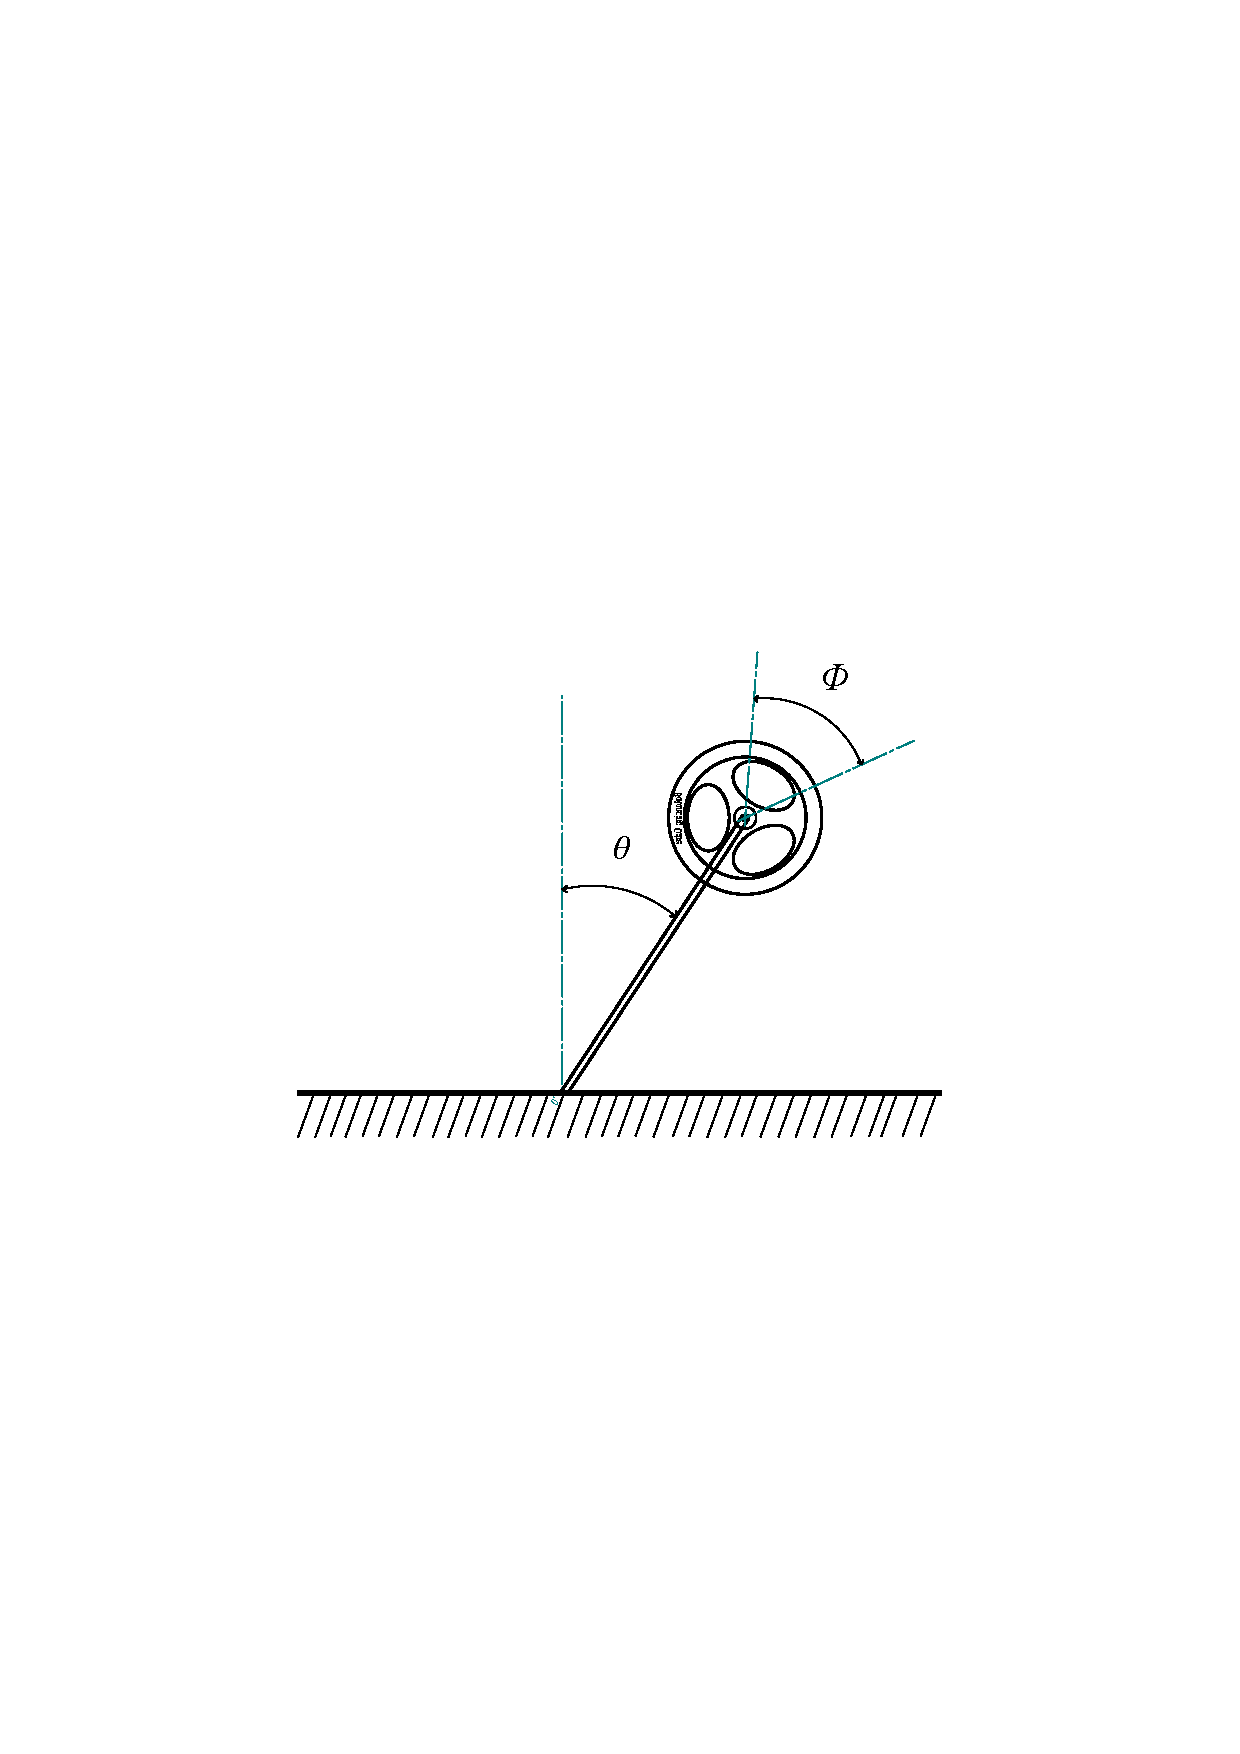
\includegraphics[trim=5cm 9cm 5cm 9cm, clip=true,scale=.6]{Lagrangeflywheel2.pdf}
\caption{Cube modelled as a reaction wheel pendulum }
\label{fig:Lagrangeflywheel}
\end{figure}

\emph{Lagrangian} Dynamics have been used to derive the systems behaviour. For a described mathematical walkthrough of how the model has been deduced see appendix \ref{app: system dyn}. First of all, the cube's rotation $\theta$ is expressed by the flywheel movement $\phi$. The Lagrangian  results in a torque equation around the pivot point
\begin{equation} \label{eq:torque pivot}
M_{tot} \cdot g \cdot l \cdot \sin \theta - I_c \cdot \ddot{\theta} = I_f \ddot{\phi}
\end{equation}
By making the assumption that the cube will balance with small deviations from the equilibrium point the angle can be expressed without the sine function. By transforming equation \ref{eq:torque pivot} to the Laplace domain it is possible to express a transfer function for the flywheel angle
\begin{equation} \label{transferfunc 1}
\phi (s) = \frac{M_{tot} \cdot g \cdot l \cdot-I_c \cdot s^2}{I_f \cdot s^2}  \theta(s)
\end{equation}
As the controller input is regulated by voltage a relation between voltage and flywheel angle has to be determined. The torque exerted on the flywheel depends on the current flowing through the motor as well as gearing and efficiency of the components
\begin{equation} \label{eq: motor torque1}
I_f \cdot \ddot{\phi} \cdot \eta_m \cdot \eta_g \cdot \Gamma = K_t \cdot i
\end{equation}
Using the voltage across the motor poles, the equation \ref{eq: motor torque1} can be written as

\begin{equation} \label{eq: laplace almost}
I_f \cdot \ddot{\phi} \cdot \eta_m \cdot \eta_g \cdot \Gamma = K_t \frac{U - \dot{\phi} K_e}{R}
\end{equation} 

By transforming equation \ref{eq: laplace almost} to the Laplace domain and combining it with equation \ref{transferfunc 1} a complete transfer function can be derived which express how the cube's angle depends on the input voltage in the Laplace domain
\begin{equation} \label{eq: laplace system}
\theta(s) = \frac{K_t \cdot I_f \cdot \eta_m \cdot \eta_g \cdot \Gamma \cdot s^2}{R_a (M_{tot} \cdot g \cdot l - I_c \cdot s^2)(I_f \cdot s^2 + \frac{K_t \cdot K_e \cdot s}{R_a})} U(s)
\end{equation}

With the transfer function from equation \ref{eq: laplace system} initial PID-parameters for the demonstrator could be estimated.

 

 
\chapter{Design and implementation} \label{chapter: demonstrator}
\epigraph{\textit{"It is impossible to make anything foolproof, because fools are so ingenious."}}{Murphy's law}


This part covers the design of the demonstrator and the motivation of components. As well as how the theory introduced in chapter \ref{chapter: theory} was implemented.

\section{Problem Formulation}
The construction of the cube can be seen as an engineering problem. The cube should be a robot that,
using a reaction wheel can balance on its edge. All components were mounted in the robot, then only requiring a power source. 

The main components consisted of a frame, reaction wheel, motor, motor controller, Arduino, and an IMU.


The goal of this project was to build a structure which remain stable in an unstable condition. A process of this sort can be divided into several parts. 
\begin{itemize}
\item Design
\item Motor Control
\item Sensor Reading
\item System Control
\end{itemize}
All these individual systems had to be implemented and joined in the final assembly.

\section{Design}

\subsection{Frame}
The construction problem was to decide the size of the cube and reaction wheel. A heavier construction with more inertia results in a pendulum which is simpler to stabilize. But also demands a larger torque and thus a more powerful motor which in turn requires another controller.

The frame of the cube was constructed in aluminium consisting of 3 plates. By keeping the heavy parts symmetric considering the electrical components, the subsystems could be placed arbitrarily and the center of gravity still assumed to be in the center of the cube. By constructing the cube in such a way the mathematical model was easier to derive.

The final design is seen in Figure \ref{Fig: final design}. The motor was fixed through the middle wall, the shaft on one side and the body on the other. The motor controller and microcontroller fastened at the backplate whilst the sensor is placed on the front, to be moved during the research.



\begin{figure}[!htb]
\centering
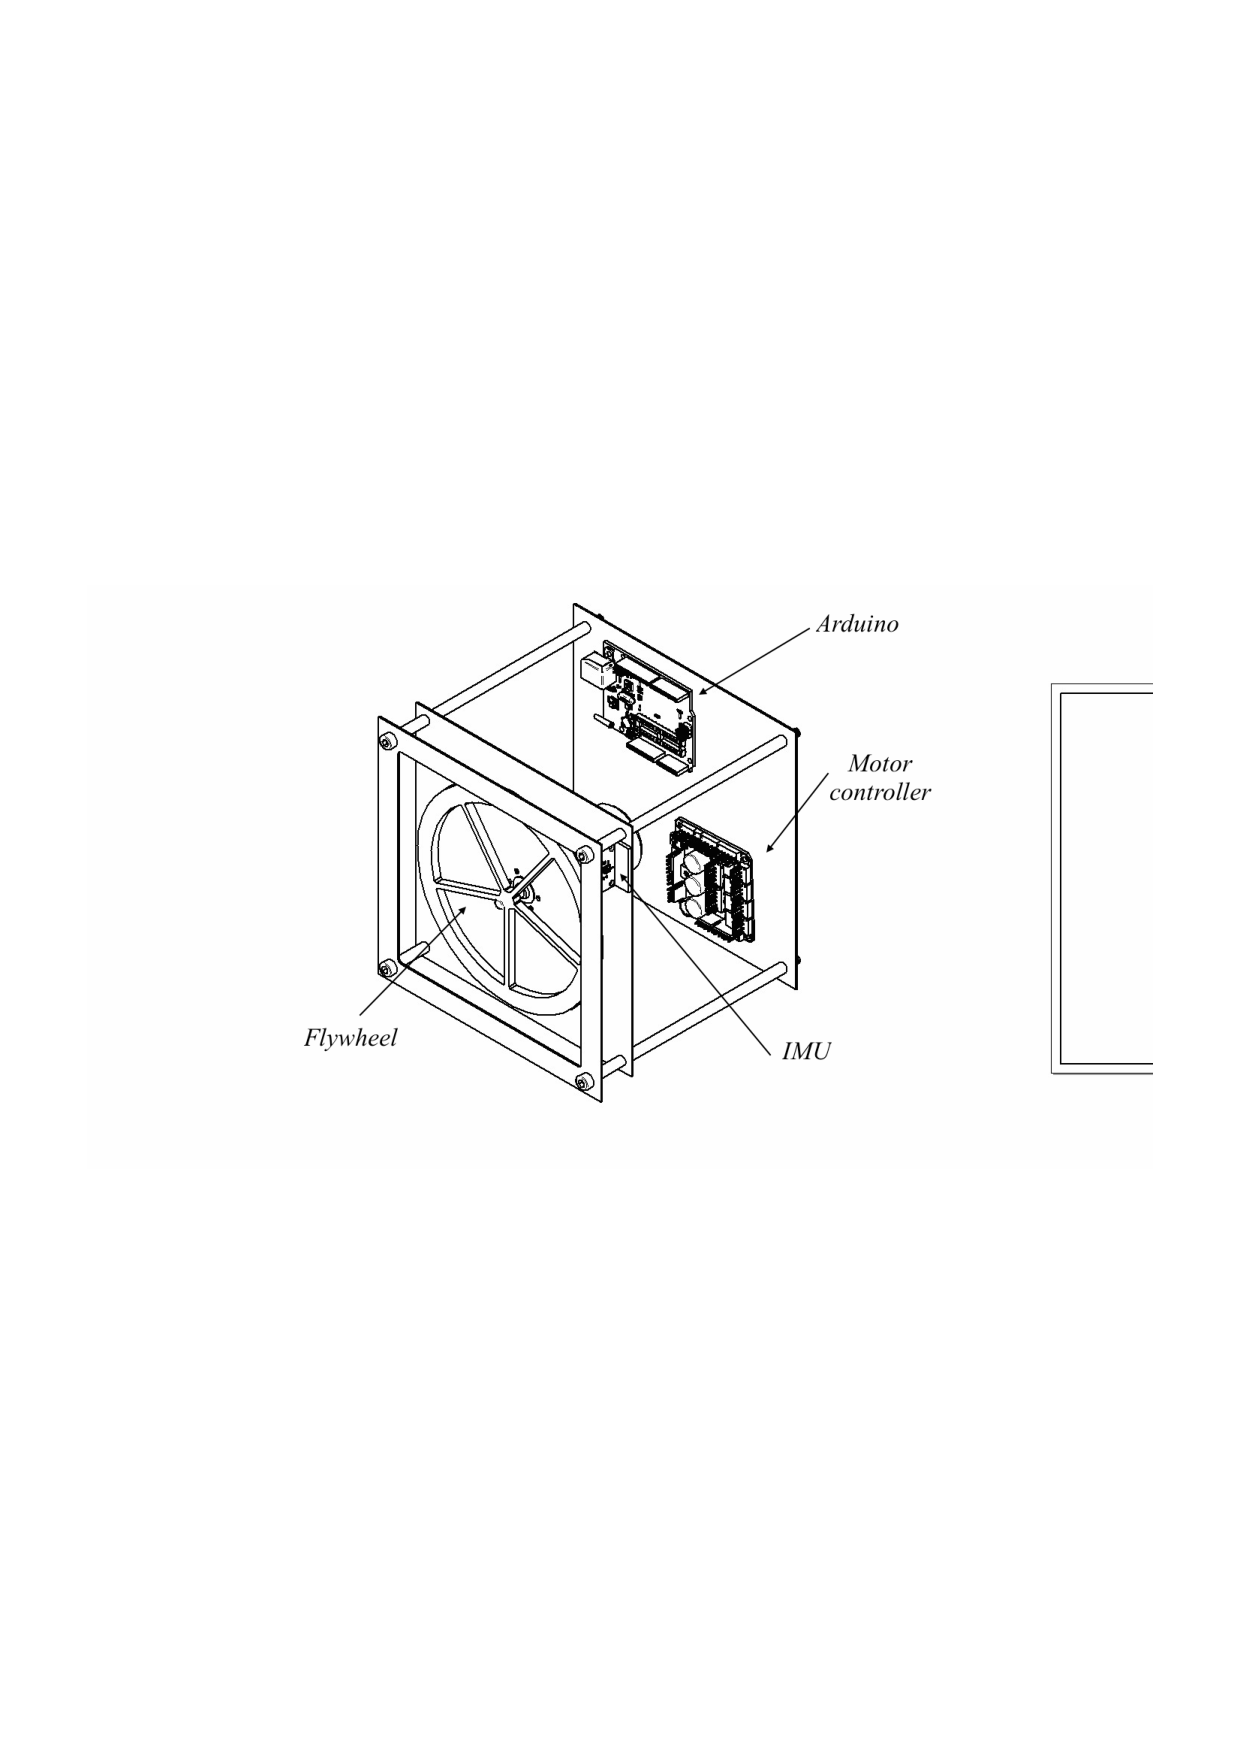
\includegraphics[trim=5cm 10cm 5cm 9cm, clip=true,scale=.9]{Finaldesign.pdf}
\caption{The final design of the cube}
\label{Fig: final design}
\end{figure}

\subsection{Arduino}
The Arduino is an open source, 8-bit microcontroller that was used in the robot. 
The board run on 5 and 3.3 volts and has outputs for both. This was used to power both the IMU and the motor controller, external power only had to be used for the motor main supply.

\subsection{Motor controller}
A factory made full H-bridge DC motor controller on a chip was used. The main criteria the controller had to meet was current and voltage capabilities suitable for the motor. A motor controller from Pololu was used specified at 28V and able to handle continuous currents of three ampere. The chosen controller also had a safety function that disabled the motor if an over-current ran through the controller.

The motor controller was connected to the Arduino, with 4 cables, each for a different functionality. PWM signal input, a brake function input, a direction switch input and an status flag output. A schematic diagram of all these connections can be seen in appendix \ref{app: electrical circuit}

\subsection{Motor}
To apply torque to the flywheel, a Maxon DC motor with a nominal voltage of 24V was used. The torque excerted on the flywheel is correlated to the ability to balance the cube at a larger deviation from the center-line. To gain a large torque but still maintaining a current that the motor controller could handle a spur gear with a ratio of 10 was used. 

\section{System analysis}
To analyse how the system behaves the transfer function obtained from equation \ref{eq: laplace system} is used
\begin{equation}\label{eq: transfer function final}
G(s) = \frac{K_t \cdot I_f \cdot \eta_m \cdot \eta_g \cdot \Gamma \cdot s^2}{R_a (M_{tot} \cdot g \cdot l - I_c \cdot s^2)(I_f \cdot s^2 + \frac{K_t \cdot K_e \cdot s}{R_a})} 
\end{equation}

Figure \ref{Fig: PZ & RootLocus} shows the Pole-Zero map and Root locus of the system indicating that the system is unstable in the open loop system. \cite{regler} To evaluate if the closed loop system is stable with a scalar gain $K$, Root Locus in Figure \ref{Fig: RootLocus} is used which indicates that the system is unstable.


\begin{figure}
\centering
\begin{subfigure}{.5\textwidth}
  \centering
  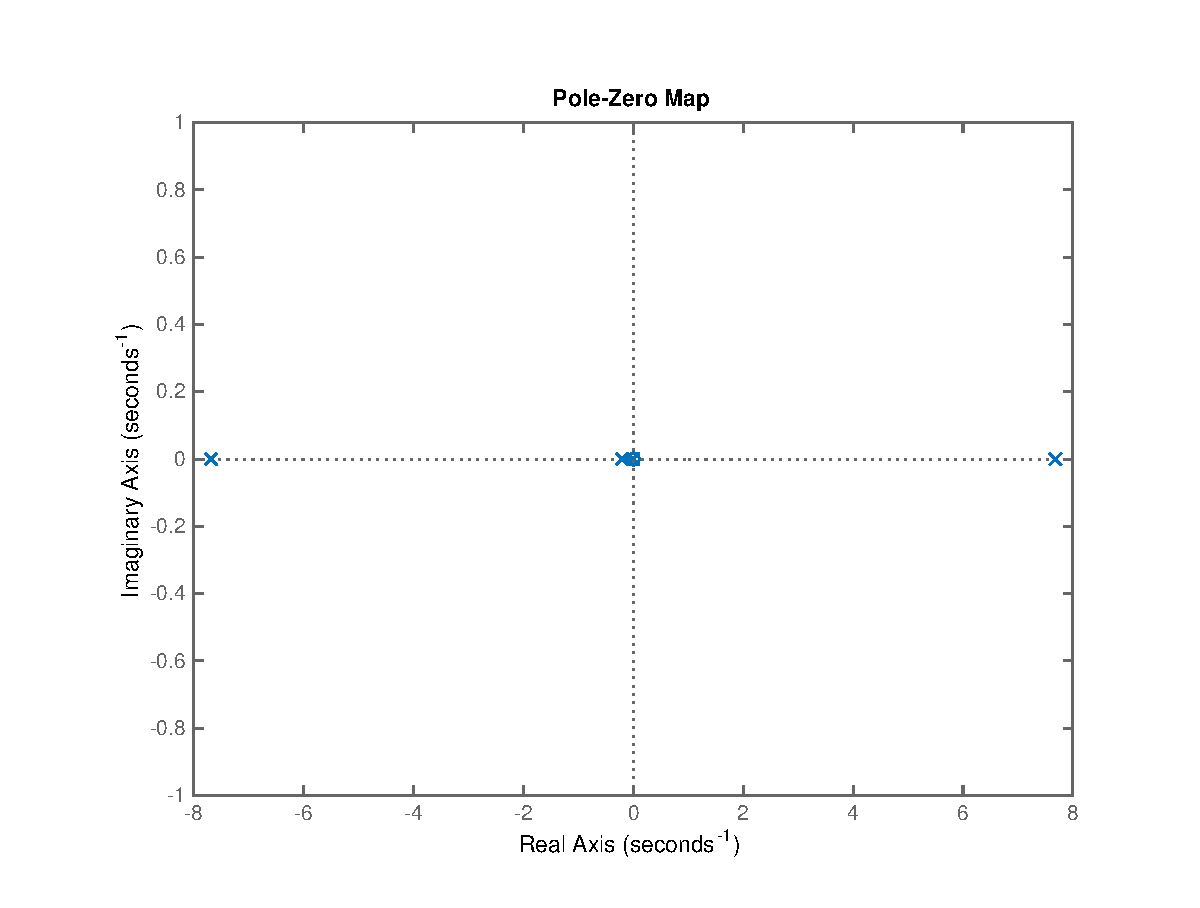
\includegraphics[width=\textwidth]{PzMap.eps}
  \caption{Pole Zero map}
  \label{Fig: PZmap}
\end{subfigure}%
\begin{subfigure}{.5\textwidth}
  \centering
  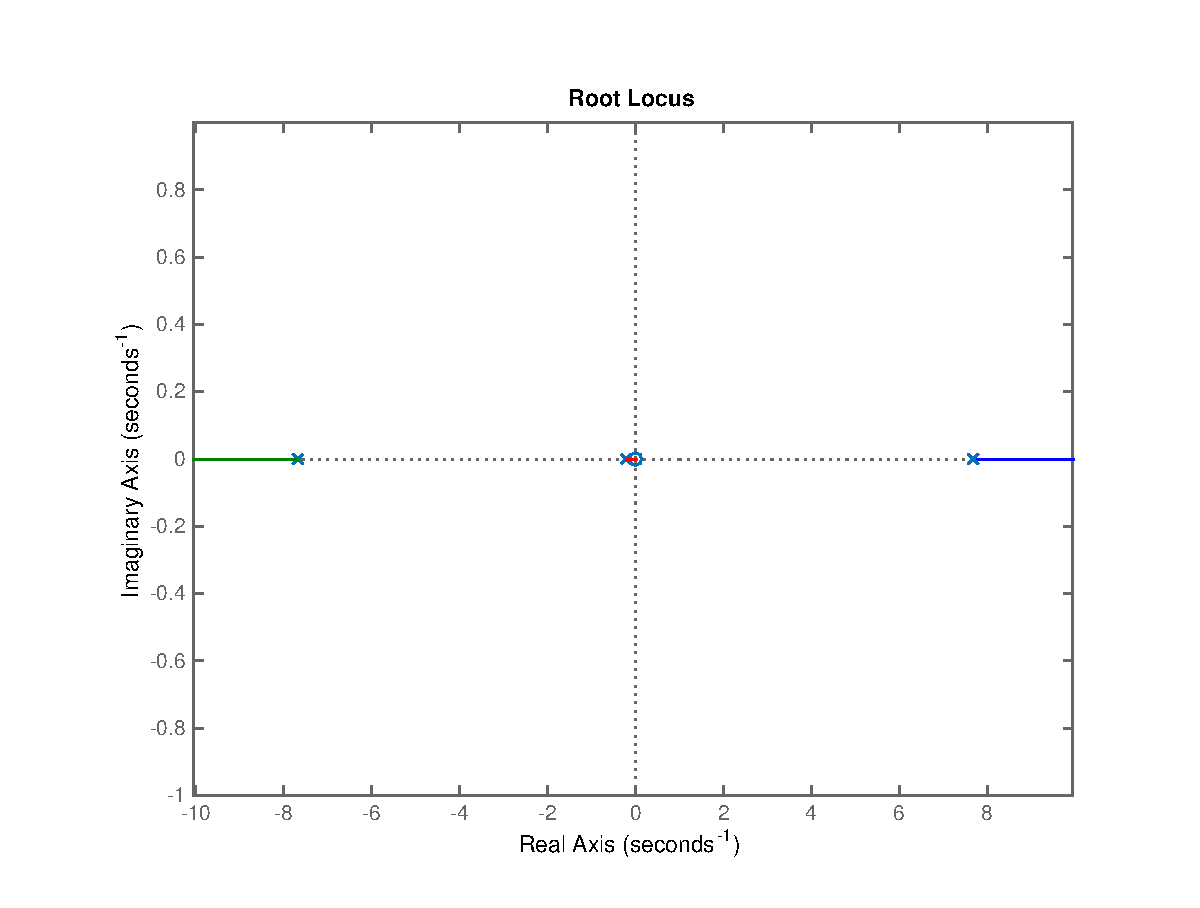
\includegraphics[width=\textwidth]{RootLocus.eps}
  \caption{Root Locus}
  \label{Fig: RootLocus}
\end{subfigure}
\caption{A figure with two subfigures}
\label{Fig: PZ & RootLocus}
\end{figure}

Matlab was then used to estimate rough proportions of the PID values. To be fine tuned during experiment.


\section{Software}
All software was run on the Arduino microcontroller and all code were written in the Arduino environment. The Arduino \textit{integrated development} (IDE) use the extension .ino but the code is written in a combination of C and C++.

All other calculations to examine the system and performance figures was made using MATLAB.

\section{Inertial navigation system}

\subsection{Inertial measurement unit}
The sensor used was a 9-DOF MPU-9150 from Sparkfun. As sensitivity was preferred and considering that the cube does not rotate around the pivot point at high velocities the gyroscope range was set to lowest possible 250 deg/s and thus keeping a sensitivity of 131 LSB's/dps


\subsection{Kalman implementation}
For the implementation of Kalman filter a library made by Lauszus was used, which is available a the Github repository \cite{TKJkalman}. For an extended explanation of the Kalman implementation, see appendix \ref{app: Kalman imp}.

\begin{figure}[!htb]
\centering
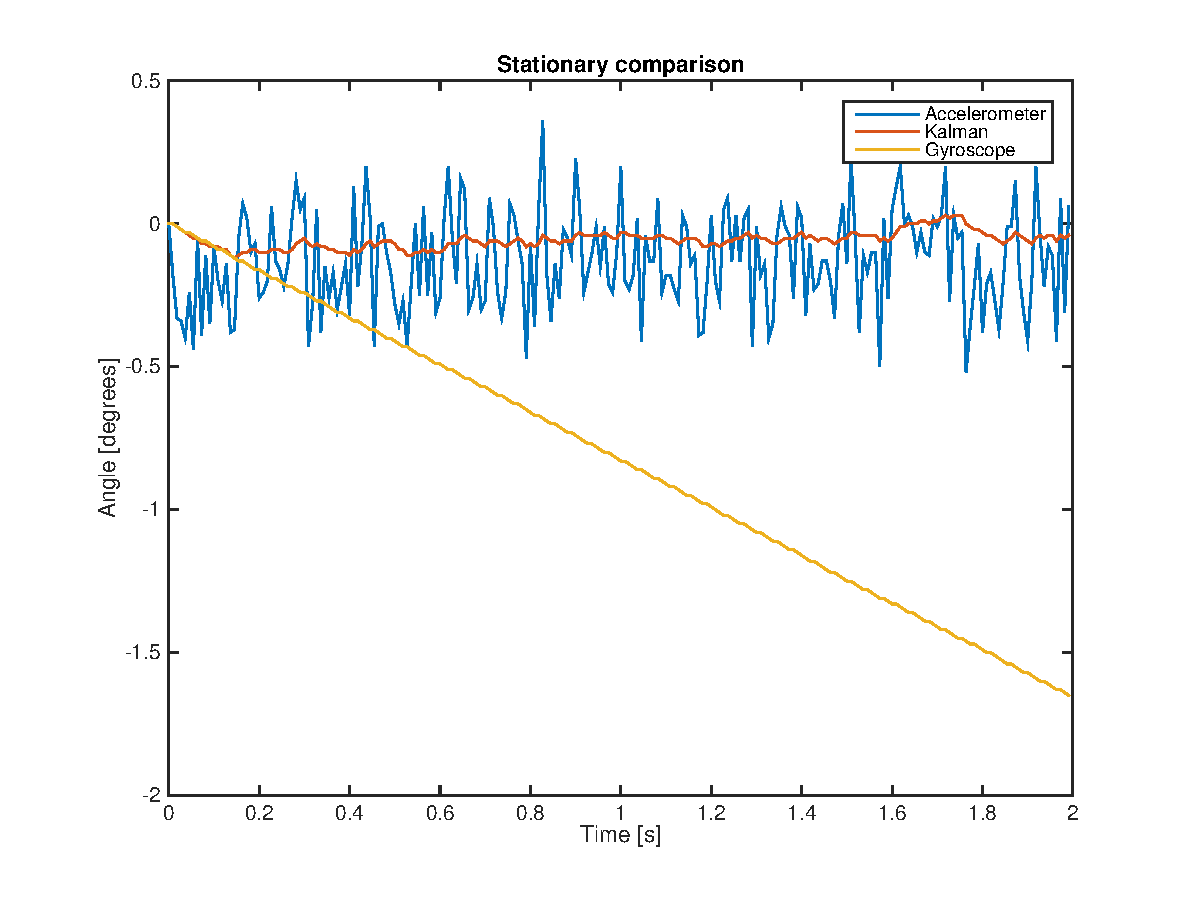
\includegraphics[scale=0.6]{Stationarycomparison.eps}
\caption{Comparison of Kalman filtered-, gyroscope- and accelerometer angle}
\label{Fig: Kalman comparison}
\end{figure}
Figure \ref{Fig: Kalman comparison} shows a comparison of the estimated angle at a stationary position using the gyroscope, accelerometer and the Kalman filtered signals separately. The estimated angle using only the gyroscope can be seen as the negative angle ramp. This is due to the bias error that is being integrated. The accelerometer readings show that the signal contains a lot of white noise but still has a mean value of zero. 
The Kalman filtered angle starts converging to the gyroscope measurements but are then corrected when weighed against the accelerometer which can be seen early in the plot. 
This indicates that the Kalman filter works but the estimated state should still not be considered as \textit{true}. 
\begin{figure}[!htb]
\centering
\begin{subfigure}{.5\textwidth}
  \centering
  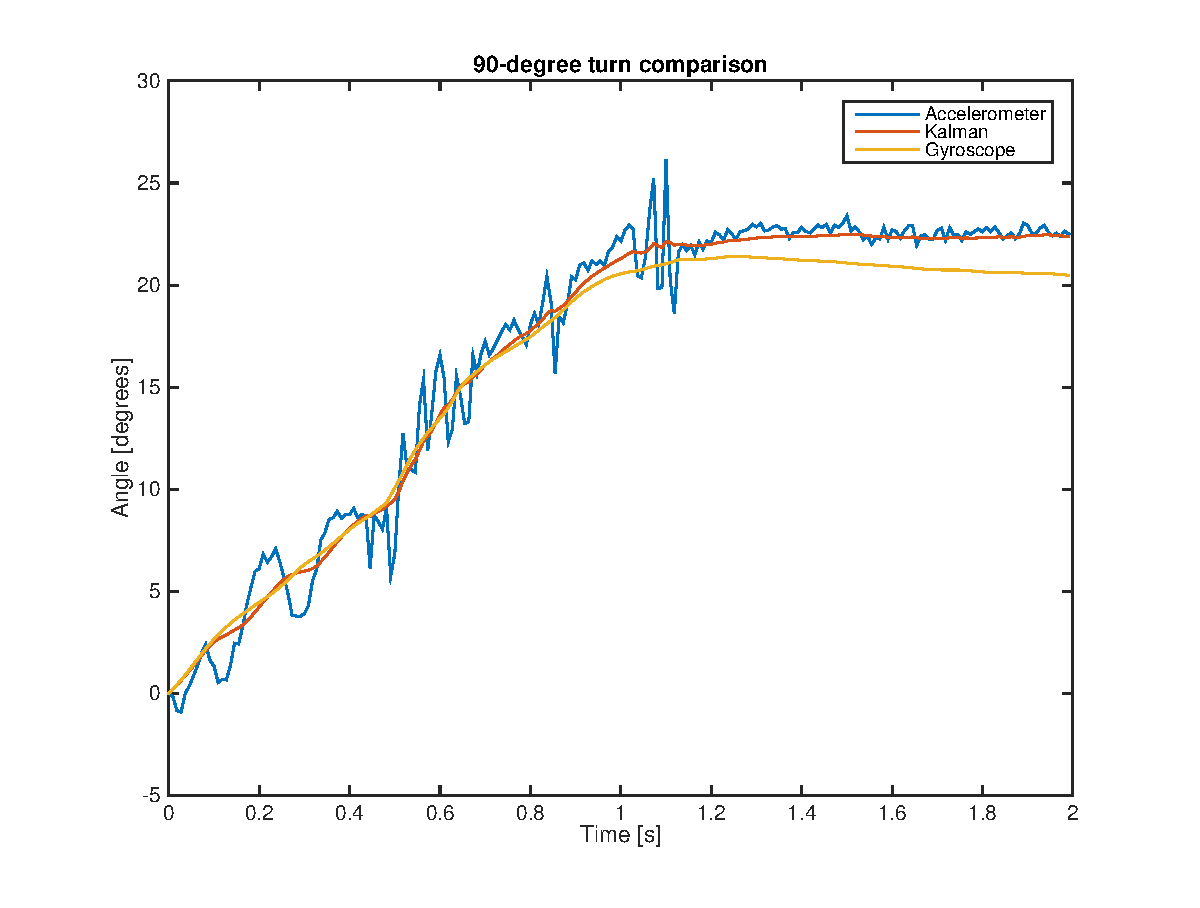
\includegraphics[width=\textwidth]{Kalmanturn.eps}
  \caption{90 degree turn}
  \label{Fig: Kalmanturn}
\end{subfigure}%
\begin{subfigure}{.5\textwidth}
  \centering
  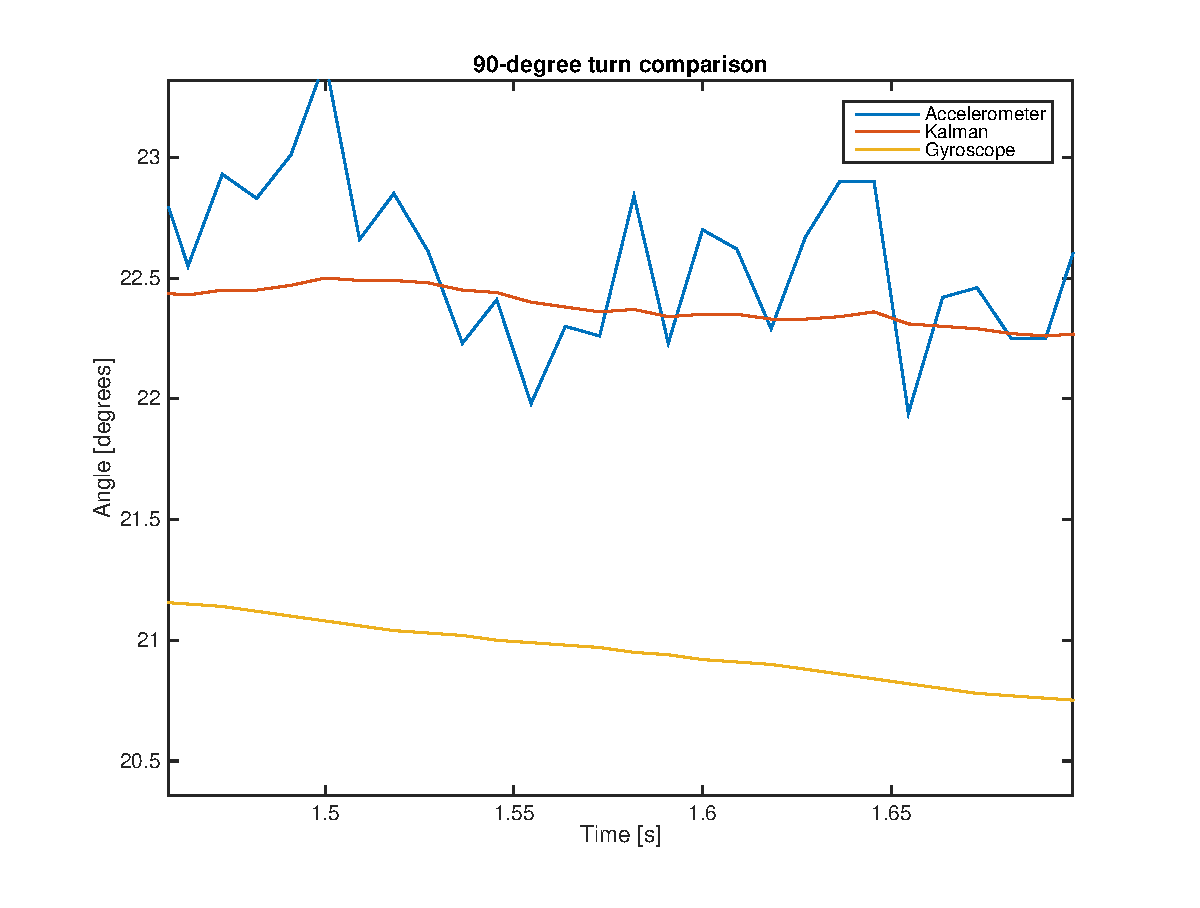
\includegraphics[width=\textwidth]{Kalmanturnzoom.eps}
  \caption{Zoomed view}
  \label{Fig: Kalmanturnzoom}
\end{subfigure}
\caption{Comparison of the estimated angle during a 90-degree turn}
\label{Fig: Kalmanturnfull}
\end{figure}

Figure \ref{Fig: Kalmanturnfull} illustrates the estimated angle during a 90 degree turn done by hand. Subfigure \ref{Fig: Kalmanturnzoom} shows a zoomed view of the plot where the gyroscope bias is distinct but the Kalman angle is converging towards the true angle.



\subsection{Measurement and process noise} \label{chapter:Allan Variance}
For the Kalman filter to properly work it is essential to know how reliable the process and measurement inputs are.  A way of determining the process noise and measurement noise of the IMU is the Allan variance method. The theory of Allan variance is outside the scope of this thesis but for reader reference is a time domain analysis technique commonly used to determine the characteristics of errors for inertial sensors\cite{Allancalibration}.
The gyroscope data is treated as an external input to the system, so the error and bias from the readings are characterised as process noise. This is then compared to the measurement, the accelerometer, which contains a measurement noise.
By gathering samples from the gyroscope and accelerometer at a stationary state the Allan variance can be calculated. The Allan variance is then used to determine the noise and stability of the system. The interesting components of the variance for the IMU are the ARW, VRV and bias stability mentioned in section \ref{section:IMU}.
Data from the gyroscope was collected during twelve hours to retrieve a reliable estimate of the bias. 
The root Allan variance was calculated and is shown in Figure \ref{fig:gyroscope allan} where the variance is a function of averaging time $\tau$

\begin{figure}[!htb]
\centering
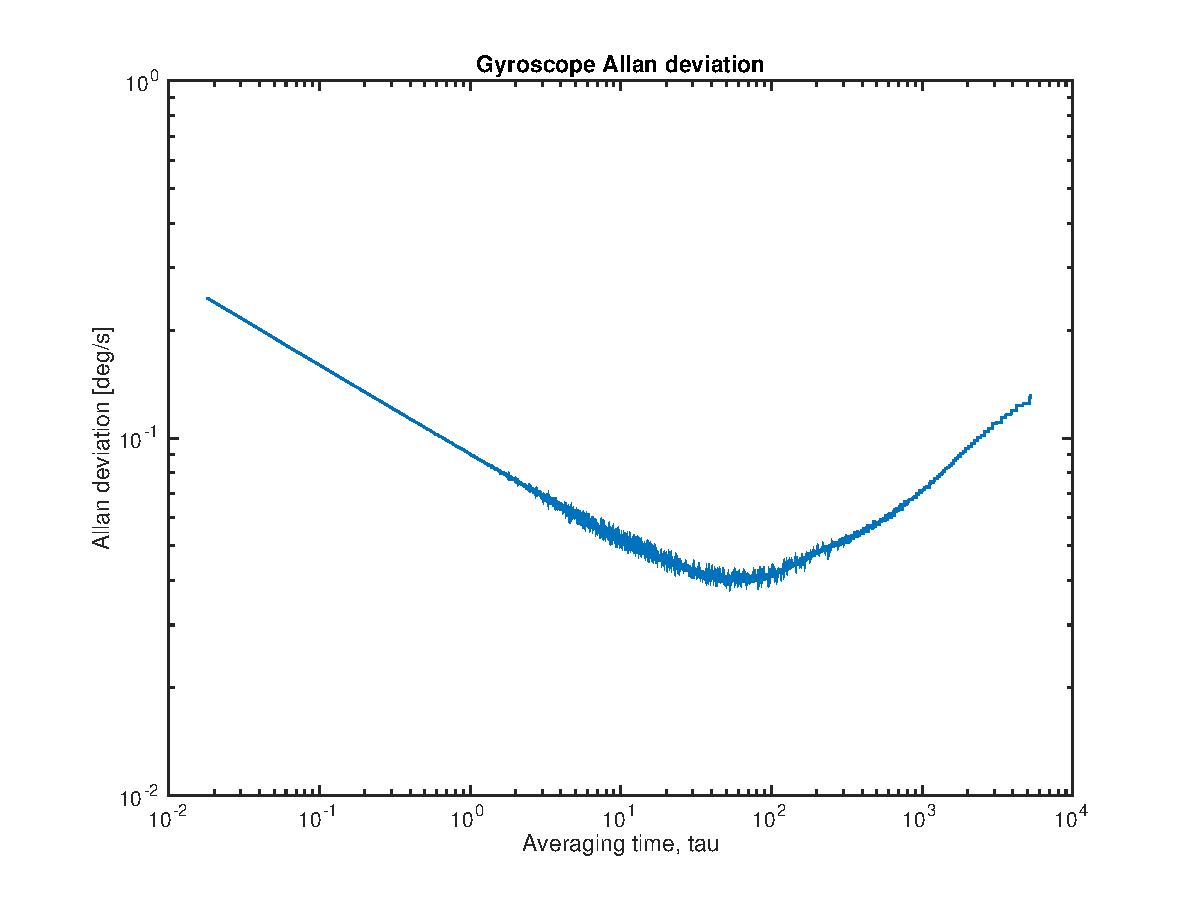
\includegraphics[scale=.6]{gyroscopeallan.eps}
\caption{Gyroscope root Allan variance}
\label{fig:gyroscope allan}
\end{figure}

The angle (or velocity, concerning the accelerometer) random walk can be depicted from the plot at an angle of -0.5 while the bias instability is determined by looking at the lowest point of the plot. Allan variance for the accelerometer was retrieved in a similar manner.  The results can be seen in table \ref{Table: Allan variance}.

\begin{table} [!hbt]
\centering
\begin{tabular}{@{}cc@{}} \toprule
Noise term & Degrees/second\\ \midrule
Angle random walk  	 & 0.00905\\
Bias stability   & 0.00395\\
Velocity random walk  	 & 0.014\\
\bottomrule
 \end{tabular}
 \caption{Allan variance results }
  \label{Table: Allan variance}
\end{table}




These values corresponds to the process and measurement noise covariance matrices used by the Kalman filter \ref{eq:covariance process noise} and \ref{eq:covariance measurement noise}.



%\section{System Control}
%The choosen control method was a \textit{Proportional Integration Derivative} (PID) regulator. This was because no feedback was taken from the motor. The parameters for the PID were both experimentally determined and calculated with MATLAB. The MATLAB's PID-tuner did not perform as well as the experimental values so those were used.
%
%Any implemented control system is discrete which means cation has to be taken when the applied model is in continuous domain. Foremost the sampling frequency, which is crucial. If the sampling frequency is to low the system response might not detect changes fast enough or behave unexpectedly. According to the Nyquist criteria the Nyquist frequency $f_n$ and sampling frequency $f_s$
%is
%\begin{equation}
%f_n<=2 \cdot f_s
%\end{equation}.
%The signal must be filters´d to remove the i´unwanted frequencies. In the cube the sample frecuency \textbf{IN MED TROLL OM VARFÖR VI UPPFYLLER HÄR}
%
%The best parameters for the PID was
%\textbf{KANSKE EN TABELL HÄR}
%These parameter are dependant on both the demostrator and the program code as are not general. The proportional parameter value was determined first. When a overshootal behaviour was found the other parameters were also determined.
\section{Electronics}



\subsection{PWM}
The PWM frequency was set to 20KHz, the maximum the motor controller can cope with \cite{MC33926}. The duty cycle was varied during the program and calculated from the control system. A typical PWM signal, with 80 \%  duty can be seen in Figure \ref{Fig: PWMscope} as the upper signal. The lower signal is the one applied to the motor.

A more in depth explanation of the PWM implementation can be found in the appendix \ref{app: PWM}.
\begin{figure}[!hbt]
\centering
\includegraphics[trim=5cm 5.5cm 5cm 5cm, clip=true,scale=0.15]{PWMpic1.jpg}
\caption{PWM, signal from Arduino and applied on motor}
\label{Fig: PWMscope}
\end{figure} 


\chapter{Results}
The first test was conducted during a stationary condition only moving the IMU to the different positions as specified in section \ref{sec: method}.

The standard deviation and expected value of the IMU signal at the different placements are seen in table \ref{Table: Standard deviation}.

\begin{table} [!hbt]
\centering
\begin{tabular}{@{}llcc@{}} \toprule
\multicolumn{3}{r}{Angle} \\ \cmidrule(r){3-4}
Position & Motor & Standard deviation & Expected value\\ \midrule
A  	 & Enabled 	& 0.92 & 44.19 \\
B    & Enabled 	& 0.87 & 44.44 \\
C  	 & Enabled 	& 0.59 & 44.26\\
D   	 & Enabled 	& 0.52 & 44.00\\
E	 & Enabled 	& 0.42 & 44.15\\
	 & Disabled	& 0.11 & 44.40\\ \bottomrule
 \end{tabular}
 \caption{Stationary IMU data results}
  \label{Table: Standard deviation}
\end{table}

A comparison of the worst case scenario and the best measurement from position D and E can be seen in Figure \ref{Fig: Result1}

\begin{figure}[!htb]
\centering
\begin{subfigure}{.5\textwidth}
  \centering
  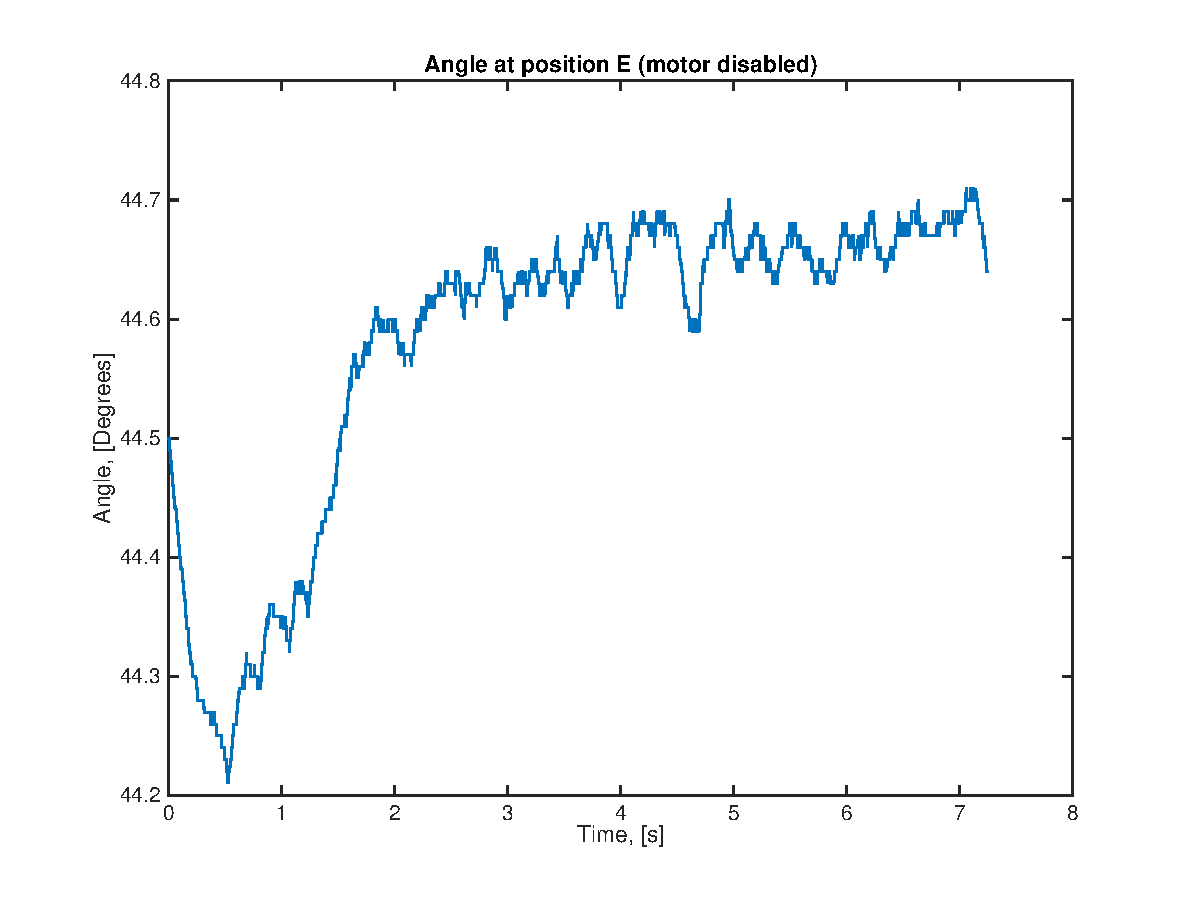
\includegraphics[width=\textwidth]{result1.eps}
  \caption{IMU angle, disabled motor}
  \label{Fig: diabled motor}
\end{subfigure}%
\begin{subfigure}{.5\textwidth}
  \centering
  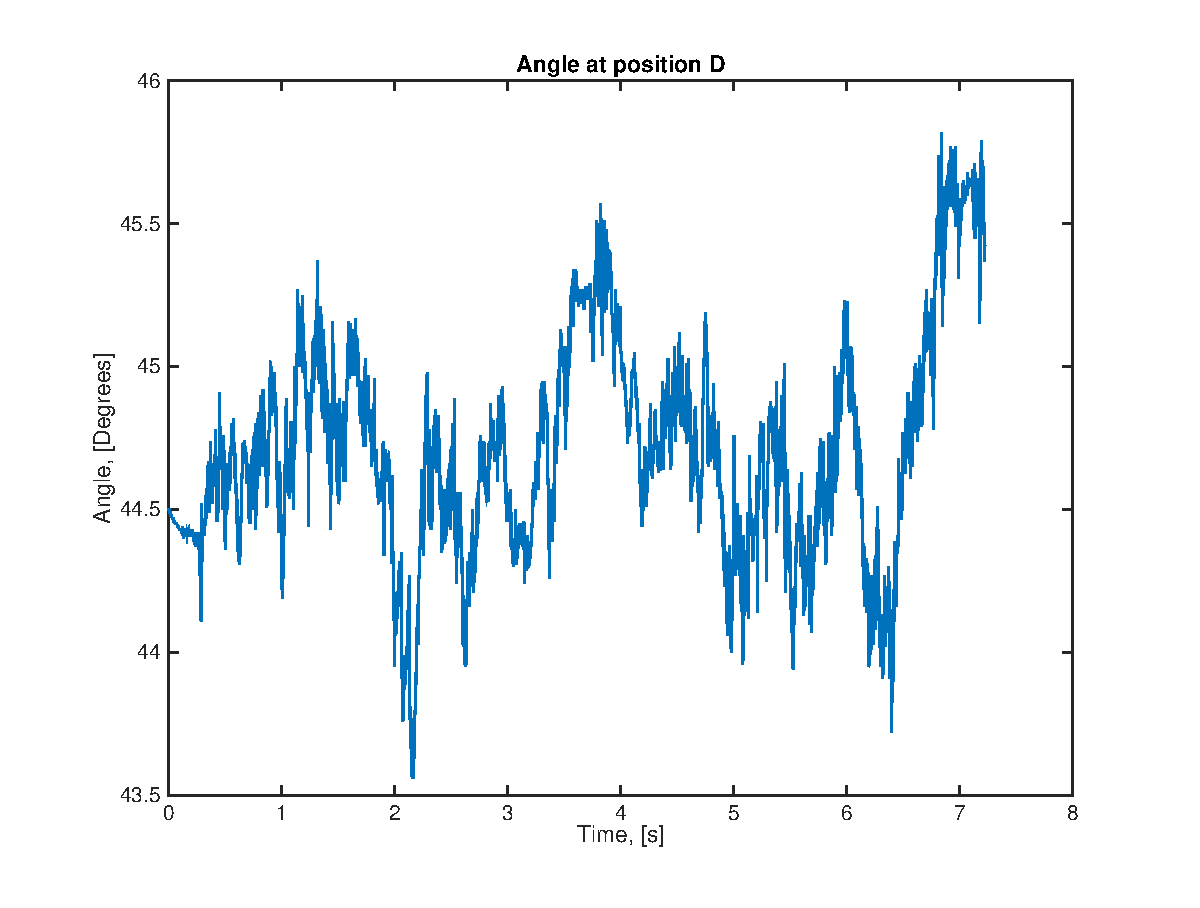
\includegraphics[width=\textwidth]{result2.eps}
  \caption{IMU angle, motor enabled}
  \label{Fig: enabled motor}
\end{subfigure}
\caption{IMU angle during stationary test}
\label{Fig: Result1}
\end{figure}

Furthermore position D and E were planned to be evaluated when balancing, to test system performance for different sensor positions. But since the cube did not balance long enough to render any unambiguous results these tests were not conducted.

\chapter{Discussion and conclusions}

\section{Discussion}
At first the sensor data was tested for different positions as described in section \ref{sec: method}. The results seen in Table \ref{Table: Standard deviation} and clearly shows that the closer the IMU was placed to the center of the cube, the standard deviation of the signal during a stationary state decreased. From this, the original hypothesis that the motor would induce an electromagnetic disturbance could be discarded.

Rather, for this setup, with a small motor, the quality of the sensor data was more inflicted by the vibrations in the structure. By placing the sensor closer to the center of the structure the standard deviation decreased. The center where the motor is mounted was more rigid and potentially dampens the vibrations.

The variations in the expected value is interesting as well. There are no relationship between the values and their respective positions. No obvious conclusion can be drawn from the expected values. Nor can we measure the correct value or even comment on what it should be, other than close to 45 degrees. Still it is important that the value is close to the real world otherwise the IMU might perceive a displaced balance point and thus having troubles balancing.
\\ 

The worst position was position A, the one on the front of the cube. At that position the IMU was close to the rotating reaction wheel. The reaction wheel itself is made of steel, a conductive and magnetic metal. This might contribute to the noise experienced by the sensor. This and the fact that it is far from the centre is the reason that it performed worse than all other tested positions.

The cube could not balance and was unstable for every sensor position. Probably not because of the sensor placement but due to the control system and design as a whole. Still it is clear from the result that sensor placement is important and that some positions are better than others.


If a bigger cube were built with a larger inertia the system would be slower and hence not require as fast control system. As for now, the gear used was a spur gear causing a slight delay when switching directions. This is something that implicates things as the system was not as responsive as required. 


\section{Conclusions}
For a construction like the one used in this project with a rather small motor the electromagnetic induction from the motor had a negligible effect on the sensor, thus should the sensor be placed only considering the vibrations in the structure. Also avoid positions close to rotating metal structures. 

Since the cube did not balance, a more powerful motor or efficient gearing would have been favourable. Though increasing the size of the motor could make the results invalid. To actually achieve balance a faster system with more torque would have been needed.


\chapter{Recommendations and future work}

\section{Recommendations}


A larger motor with higher stall torque is better for the task, as long as a suitable motor controller is used. Also an encoder to measure motor RPM is an advantage if a better control system is to be devised. Although a larger motor might induce higher currents which could render the sensor placement results unfavourable.

Regarding the microcontroller something faster than the Arduino is preferred to ease the implementation of the control system.

Also if a more extensive project is desired, a research with non-linear control systems has been done at ETH, with the name Cubli\cite{cubliECC13}, which was the inspiration of this project.

\section{Future work}
To get a preciser result regarding the IMU position, more parameters should be properly examined. Various motors and motor controllers that allow different amounts of induced currents should also be varied. If the current is measured separately its contribution could be determined independent from the vibration disturbance as well.
To investigate the system performance it is of importance to achieve balance for more than a couple of seconds, this might be the main focus.

The control system can be extended by adding features to the robot, such as making it able to jump up from a stationary state. This would require an external brake if not the motor is powerful enough to stop the reaction wheel. Something as a mechanical lock that instantly locks the reaction wheel is the most simple solution but a v-brake with two brake-callipers similar the ones used for bicycles is preferable. 

An extension of the project would also be balancing the cube not only on it's edge but it's corner. To achieve this multiple reaction wheels must be used and a more complicated control system due to changes in moment of inertia caused by angular velocities in the other reaction wheels.


%\bibliography
\cleardoublepage
\bibliography{FiM_references}
\bibliographystyle{apalike-url}%apalike-url}

\cleardoublepage
\appendix
\addtocontents{toc}{\protect\contentsline {part}{Appendices}{}{}}


\chapter{Additional information} \label{appA}
\section{The Kalman filter} \label{app: Kalman}
\subsection{Mathematical background}
To understand this recursive filter which use old and new values a \textit{a priori} and \textit{a posteriori} state is defined
\begin{equation} \label{eq: priori state}
\hat{x}^-_k
\end{equation}
\begin{equation} \label{eq: posteriori state}
\hat{x}_k
\end{equation}
The \textit{a priori}  state in equation \eqref{eq: priori state} is defined as the estimate of the current state at the time $k$. The \textit{a posteriori} state \eqref{eq: posteriori state} is the new estimated state.
For the Kalman filter to work properly some criteria has to be fulfilled. The average value of the measurement noise $z$ and process noise $w$ earlier mentioned in section \ref{section: Kalman} has to be zero, i.e. a Gaussian error. $z$ and $w$ also has to be independent of  each other. The noise and error in an IMU and many other devices have the characteristics of Gaussian noise.




During the \textit{predict} phase the filter estimates the states using the inputs from the process, i.e the gyroscope in this case. The filter then moves on to the \textit{update} phase where it compares the state to the actual measurement, the accelerometer, see Figure \ref{Fig: Kalman phases}.

Consider the true state equation \eqref{eq:kalmanstate}, first of all the Kalman filter estimates a state by neglecting the process noise
\begin{equation} \label{eq:Kalman first estimate}
\hat{x}^-_k = A\hat{x}\textsubscript{k-1}+Bu\textsubscript{k-1}
\end{equation}
As stated above the Kalman filter uses readings from both the gyroscope and accelerometer to estimate a position closer to the true value. To determine how reliable the process and measurement readings are a noise covariance is defined as
\begin{equation} \label{eq:covariance process noise}
Q = E(w_k w_k \textsuperscript{T})
\end{equation}
\begin{equation} \label{eq:covariance measurement noise}
R = E(v_k v_k \textsuperscript{T} )
\end{equation}
How to determine these covariances are further investigated in section  \ref{chapter:Allan Variance}.
From here the \textit{a priori} error covariance matrix is introduced to symbolize the noise in the process measurement
\begin{equation}
P^-_k = AP\textsubscript{k-1}A^T + Q_k
\end{equation}
During the \textit{update} phase the accelerometer measures are used. The measurement \textit{innovation} is calculated as
\begin{equation} \label{eq: innovation}
\tilde{y} = z_k - H\hat{x}^-_k
\end{equation}
The \textit{innovation} is a residual that reflects the relation between the predicted measurement and the actual measurement. A measurement \textit{innovation} of zero indicates a perfect agreement.
The measurement \textit{innovation} covariance is calculated as
\begin{equation} \label{eq:innovation cov}
S^-_k = HP^-_kH^T + R
\end{equation}
The \textit{innovation} covariance is very similiar to the \textit{priori} error covariance but represents the measurement instead. From here the core of the Kalman filter can be calculated, the Kalman gain
\begin{equation} \label{eq:Kalman gain}
K_k = P^-_kH^TS\textsuperscript{-1}_k
\end{equation}
This indicates how reliable the measurement is. Note that if the measurement covariance error \eqref{eq:covariance measurement noise} is large, the Kalman gain will be small and vice versa if the \textit{a priori} error covariance is large.
By now the \textit{a posteriori} state can be estimated
\begin{equation}
\hat{x}_k = \hat{x}^-_k + K_k\tilde{y}_k
\end{equation}
A current state has been estimated, this would be the angle used for the control loop. Finally the \textit{priori} error is updated to be used for the next \textit{a priori} error.
\begin{equation}
P_k=(I-K_kH)P^-_k
\end{equation} 
The filter now returns to the measurement phase seen in figure \ref{Fig: Kalman phases}.


\subsection{Implementation}
\label{app: Kalman imp}
The Kalman filter cycles two states, the \textit{predict} and \textit{update} phases. The filter is using discretized steps making the filter implemented on a microprocessor rather intuitive. 
An implementation of the Kalman filter on the IMU would look something like this

Consider the equation \eqref{eq:Kalman first estimate} from chapter \ref{app: Kalman} . At first the filter predicts the state
\begin{equation}
\hat{\textbf{x}}^-_k = \textbf{A}\hat{x}\textsubscript{k-1}+\textbf{B}u\textsubscript{k-1}
\end{equation}

Where

\begin{equation}
\textbf{x}_k = \begin{bmatrix}
\theta \\
\dot{\theta_b}
\end{bmatrix}_k
u\textsubscript{k-1} = \dot{\theta}
\end{equation}

\begin{equation}
\textbf{A} = \begin{bmatrix}
1  & -\Delta t \\
0   & 1
\end{bmatrix}
,
\textbf{B} = \begin{bmatrix}
\Delta t \\ 0
\end{bmatrix}
\end{equation}

The states used here  are the angle as well as the bias. Next up is the \textit{a priori} error covariance
\begin{equation}
\textbf{P}^-_k = \textbf{A} \textbf{P}\textsubscript{k-1}\textbf{A}^T + \textbf{Q}_k
\end{equation}

\begin{equation}
\begin{bmatrix}
P\textsubscript{11} & P\textsubscript{12} \\
P\textsubscript{21} & P\textsubscript{22}
\end{bmatrix}^-\textsubscript{k} =
\begin{bmatrix}
1  & -\Delta t \\
0   & 1
\end{bmatrix}
\begin{bmatrix}
P\textsubscript{11} & P\textsubscript{12} \\
P\textsubscript{21} & P\textsubscript{22}
\end{bmatrix}\textsubscript{k-1}
\begin{bmatrix}
1 & 0 \\
-\Delta t & 1
\end{bmatrix}
+
\begin{bmatrix}
Q\textsubscript{ $\theta$ } & 0 \\
0 & Q\textsubscript{$\dot{\theta}_b$}
\end{bmatrix}
\Delta t
\end{equation}

The innovation covariance mentioned in \ref{eq:innovation cov}

\begin{equation} 
\textbf{S}_k=
\begin{bmatrix}
1 & 0
\end{bmatrix}
\begin{bmatrix}
P_{11} & P_{12} \\
P_{21} & P_{22} 
\end{bmatrix}^- _k
\begin{bmatrix}
1 \\ 0
\end{bmatrix}
+
R
\end{equation}
Kalman gain in equation \ref{eq:Kalman gain}
\begin{equation}
\begin{bmatrix}
K_1 \\ K_2
\end{bmatrix}_k
=
\begin{bmatrix}
P_{11} & P_{12} \\
P_{21} & P_{22}
\end{bmatrix}^-_k
\begin{bmatrix}
1 \\ 0
\end{bmatrix}
S^{-1}_k
\end{equation}

The predicted states are then updated with the weighed measures from the accelerometer

\begin{equation}
\begin{bmatrix}
\theta \\
\dot{\theta_b}
\end{bmatrix}_k
=
\begin{bmatrix}
\theta \\
\dot{\theta_b}
\end{bmatrix}_k^-
+
\begin{bmatrix}
K_1 \\ K_2
\end{bmatrix}_k
\textbf{$\tilde{y}$}
\end{equation}

And then at last the error covariance

\begin{equation}
\begin{bmatrix}
P\textsubscript{11} & P\textsubscript{12} \\
P\textsubscript{21} & P\textsubscript{22}
\end{bmatrix}\textsubscript{k} 
=(
 \begin{bmatrix}
1 & 0 \\
0 & 1
\end{bmatrix}
-
\begin{bmatrix}
K_1 \\ K_2
\end{bmatrix}_k
\begin{bmatrix}
1 & 0
\end{bmatrix}
)
\begin{bmatrix}
P\textsubscript{11} & P\textsubscript{12} \\
P\textsubscript{21} & P\textsubscript{22}
\end{bmatrix}^-_k
\end{equation}


This is done during each loop of the microcontroller to ensure that the estimated state is as near the true state as possible.

\section{Arduino PWM implementation} \label{app: PWM}
The Arduino microcontroller has a couple of different standard \textit{pulse width modulation} (PWM) modes. The standard frequencies are 490 and 980 Hz. Using a significantly higher frequency has many advantages, especially for the control system. The chosen motor controller could work in two modes, one of them being ultrasonic the other below ultrasonic. Setting the PWM frequency above the arduino standard frequency is preferably because the the motor becomes more efficient \cite{pwmeff} and the human ear can not hear frequencies above \textasciitilde 20 KHz. The Arduino Uno's maximum PWM frequency is \textasciitilde 61 KHz, when set to high the motor controller consumes power so a good setting is just above hearing range. Which the motor control can handle \cite{MC33926}. A bit of register manipulation had to be 
done to accomplish an acceptable PWM frequency.

The Arduino has 3 clocks that controls various pins and functions in the environment. The clocks, and their respective pins and bit size, are:
\begin{itemize}
\item[\textbf{Timer 0}]
controls digital pin 10 and
works in 8-bits, it also used as reference for the delay(), millis() and micros() built in functions. i.e. changing timer 0 could disturb the code if it is using these functions. 
\item[\textbf{Timer 1}]
The 16-bit timer. Controls pin 5 and 6 and has more modes of operation than the other two timers
\item[\textbf{Timer 2}]
another 8-bit timer responsible for pin 3 and 11 on the 
Arduino Uno.
\end{itemize}
Each of these timers can be set the various PWM modes individually. All timers have prescalers which divides the chips clock speed to vary the frequency of the PWM signal in rough discrete steps (the difference between the fastest and the next to fastest frequency on timer1 is 53 KHz), see AVR documentation for more info \cite{AVR}. 

When using PWM, the PWM duty cycle is used (and optionally frequency). Once the PWM duty cycle is set this works parallel to the main program loop and does not effect the main program but is rather run on a separate thread (except when changing the PWM parameters). For example this is useful when only one Arduino is used for multiple tasks, and computing time becomes expensive. 

A non inverted mode was used, 
meaning that 100\% duty cycle equals full power all the time. There are multiple modes of PWM on the Arduino. The main ones that can be choose from are fast - and phase corrected PWM. 
When using the phase correct PWM (pcPWM) a counter counts up every clock cycle until the counter reaches a compare value, \textit{TOP}. When TOP is reached the counter is reset or "set" according to the AVR 
documentation, be aware that for the method to work, the counter has to be adjusted to "set" not "clear" or "set bottom". Then the duty cycle has to be set to a value between 0 and TOP. Choosing duty to TOP/2 will yield a 50\% duty cycle. For modes where the TOP value is not specified it defaults to 0xFF or 255 in decimal.
Phase correct mode is useful when multiple PWM signal are used, but also was useful to achive the correct frequency in the particular case due to its counting mechanic.

When using the pcPWM (on timer2 in this case), mode 5, the TOP value and duty cycle for ONE of timer2's pin's are the same variable. This means that one can not change the duty 
cycle for a certain frequency. The frequency can then be explained by
\begin{equation} \label{eq: clock freq}
frequency = \frac{clock}{2 \cdot prescaler \cdot TOP}
\end{equation}

But the other pin (nr 3) is left unaffected. So if the desired PWM is 20 KHz it is done by choosing 100 
as TOP (OCR2A for timer2) and the prescaler value to 8 (TCCR2B = (1<<CS21) pin 11 will always have 50\% duty cycle at 20 KHz. The duty cycle for pin 3 can be set continuously. If another another duty cycle for pin 3
(OCR2B) is set, the frequency will be  maintained at 20 KHZ due to the TOP (OCR2A) value is left  unchanged. The disadvantage of this method is that it requires 2 pins, while only one is used. A minor price to pay for a specific frequency and reduced headache from the high pitched noise.

To choose mode, the correct WGM values should be set in the TCCR2A and TCCR2B registers. The fifth letter "2" represents timer 2. Timer 2 is 8-bit so it has a maximum of 8 modes. If instead timer 1 is 
used more modes can be chosen allowing for a greater amount of operation modes. Other Arduino boards might have a greater number of timers which allows for more than three different PWM's, with non default frequencies, being used at the same time.


\chapter{Proofs} \label{appB}

\section{System dynamics} \label{app: system dyn}
The first equations of motion for the system is derived by using Lagrangian dynamics Firstly by expressing the generalized coordinates, forces, the energy functions and Lagrangian. And from the Lagrange equation  \cite{Lagrangeref} acquire the equations of motion . Consider the Lagrangian equation

\begin{equation}
\frac{d}{dt}\left(\frac{\partial \mathcal{L}}{\partial \dot{q_i}}\right)-\left(\frac{\partial \mathcal{L}}{\partial q_i}\right) = \tau_i
\end{equation}

Where $\tau$ is the generalized force, in this case a torque. The $q$ operator is the generalized coordinate which now is an angle. The cube's angular momentum is counteracted by the flywheel and the system can be divided into two parts, One considering the movement of the cube, the other the flywheel.

\begin{equation} \label{eq:positiveL}
\tau_k=\frac{d}{dt}\left(\frac{\partial \mathcal{L}}{\partial \dot{\theta}}\right)-\left(\frac{\partial \mathcal{L}}{\partial \theta}\right)
\end{equation}

\begin{equation} \label{eq:negativeL}
-\tau_k=\frac{d}{dt}\left(\frac{\partial \mathcal{L}}{\partial \dot{\phi}}\right)-\left(\frac{\partial \mathcal{L}}{\partial \phi}\right)
\end{equation}

Whereas $\theta$ represents the angle of the cube and $\phi$ is the position of the flywheel. \\
The Lagrange equation is derived from the difference in kinetic energy and potential energy of the cube

\begin{equation} \label{eq:Lagrange}
\mathcal{L} = E_k - E_p
\end{equation}

\begin{equation} \label{eq:kinetic energy}
E_k = \frac{I_c \cdot \dot{\theta^2}}{2} + \frac{I_f \cdot \dot{\phi^2} }{2}
\end{equation}

\begin{equation} \label{eq:potential energy}
E_p = M_{tot} \cdot g \cdot l \cdot \cos \theta
\end{equation}
The Lagrangian \eqref{eq:Lagrange} is then

\begin{equation}
\mathcal{L} = \frac{I_c \cdot \dot{\theta^2}}{2} + \frac{I_f \cdot \dot{\phi^2} }{2} - M_{tot} \cdot g \cdot l \cdot \cos \theta 
\end{equation}

The kinetic energy depends on the angular velocities of the main construction as well as the flywheel fixed to the motor. Note that the total moment of inertia $I_c$ is defined around the pivot point of the cube. The potential energy has been defined as being at its maximum when the cube is balancing in an upright position. The construction is considered to be symmetric and hence the gravitational force is applied at the center of the cube.
Equation \eqref{eq:positiveL} and \eqref{eq:negativeL} with \eqref{eq:Lagrange}

\begin{equation} \label{eq:negativeL2}
I_c \cdot \ddot{\theta} - M_c \cdot g \cdot l \cdot \sin \theta   = -\tau_k
\end{equation}

\begin{equation} \label{eq:postiveL2}
I_s \cdot \ddot{\phi} = \tau_k
\end{equation}

Equation \ref{eq:negativeL2} together with \ref{eq:positiveL} express how the flywheel and main construction correlates of each other

\begin{equation}
I_c \cdot \ddot{\theta} - M_c \cdot g \cdot l \cdot \sin \theta   = -I_s \cdot \ddot{\phi}
\end{equation}
To use linear control methods the model has to be linearised. This is done at the unstable equilibrium where the cube is balancing. Consider the sinus term at the equilibrium point where $\theta$ equals $0$. The term can then be expressed with Maclaurin expansion

\begin{equation} \label{eq: sinus taylor}
sin \theta = \theta - \frac{\theta^3}{3!} +\frac{\theta^5}{5!}... \approx \theta 
\end{equation}

In the Laplace domain the flywheel angle $\phi$ can then be described by a transfer function and $\theta$

\begin{equation} \label{appeq: flywheelvscons}
\phi (s) = \frac{M_{tot} \cdot g \cdot l \cdot-I_c \cdot s^2}{I_f \cdot s^2}  \theta(s)
\end{equation}

The transfer function that explains of $\phi$ as a function of $\theta$ is then

\begin{equation} \label{appeq: transferfunc1}
G_1(s) = \frac{M_{tot} \cdot g \cdot l \cdot-I_c \cdot s^2}{I_f \cdot s^2} 
\end{equation}

As the controller input is voltage, the angle of the cube has to be expressed with a voltage input.
The torque exerted on the flywheel is described by the current flowing through the motor as well as the motor and gear efficiency

\begin{equation}\label{eq: Motor torque}
I_f \cdot \ddot{\phi} \cdot \eta_m \cdot \eta_g \cdot \Gamma  = K_t \cdot i
\end{equation}

The voltage across the two poles of the motor can be circumscribed by the current flowing through a motor
\begin{equation} \label{appeq: motor voltage}
U = L\frac{di}{dt} + iR + \dot{\phi}K_e
\end{equation}
Equation \ref{appeq: motor voltage} and \ref{eq: Motor torque} gives 

\begin{equation} \label{eq:motor torque}
I_f \cdot \ddot{\phi} \cdot \eta_m \cdot \eta_g \cdot \Gamma = K_t \cdot \frac{U-E_{\text{emf}} }{R_m}
\end{equation}

Note that the motor inductance in neglected in equation \eqref{eq:motor torque}, that is due to the inductance time constant which is fast considering the rest of the system and is not vital for the control system \cite{KTHpendulum}.
The induced voltage can be described as a function of motor speed.

\begin{equation} \label{eq: induced voltage}
E_{\text{emf}} = K_{\text{emf}} \cdot \dot{\phi_r}
\end{equation}
By moving to the Laplace domain and combining equations \ref{eq:motor torque}, \ref{eq: induced voltage}, \ref{appeq: flywheelvscons} and \ref{appeq: transferfunc1} one gets

\begin{equation}
I_f \cdot \eta_m \cdot \eta_g \cdot \Gamma \cdot G_1(s) \cdot s^2 + \frac{K_t \cdot K_e \cdot s}{R_a} \theta(s) = \frac{Kt}{R} U(s)
\end{equation}
And at last the cube's angle in the Laplace domain can be described by a transfer function and the voltage input $U$
\begin{equation}
\theta(s) = \frac{K_t \cdot I_f \cdot \eta_m \cdot \eta_g \cdot \Gamma \cdot s^2}{R_a (M_{tot} \cdot g \cdot l - I_c \cdot s^2)(I_f \cdot s^2 + \frac{K_t \cdot K_e \cdot s}{R_a})} U(s)
\end{equation}

\chapter{Schematics} \label{appC}
\section{Electrical circuit}
\label{app: electrical circuit}
\begin{figure}[!htb]
\centering
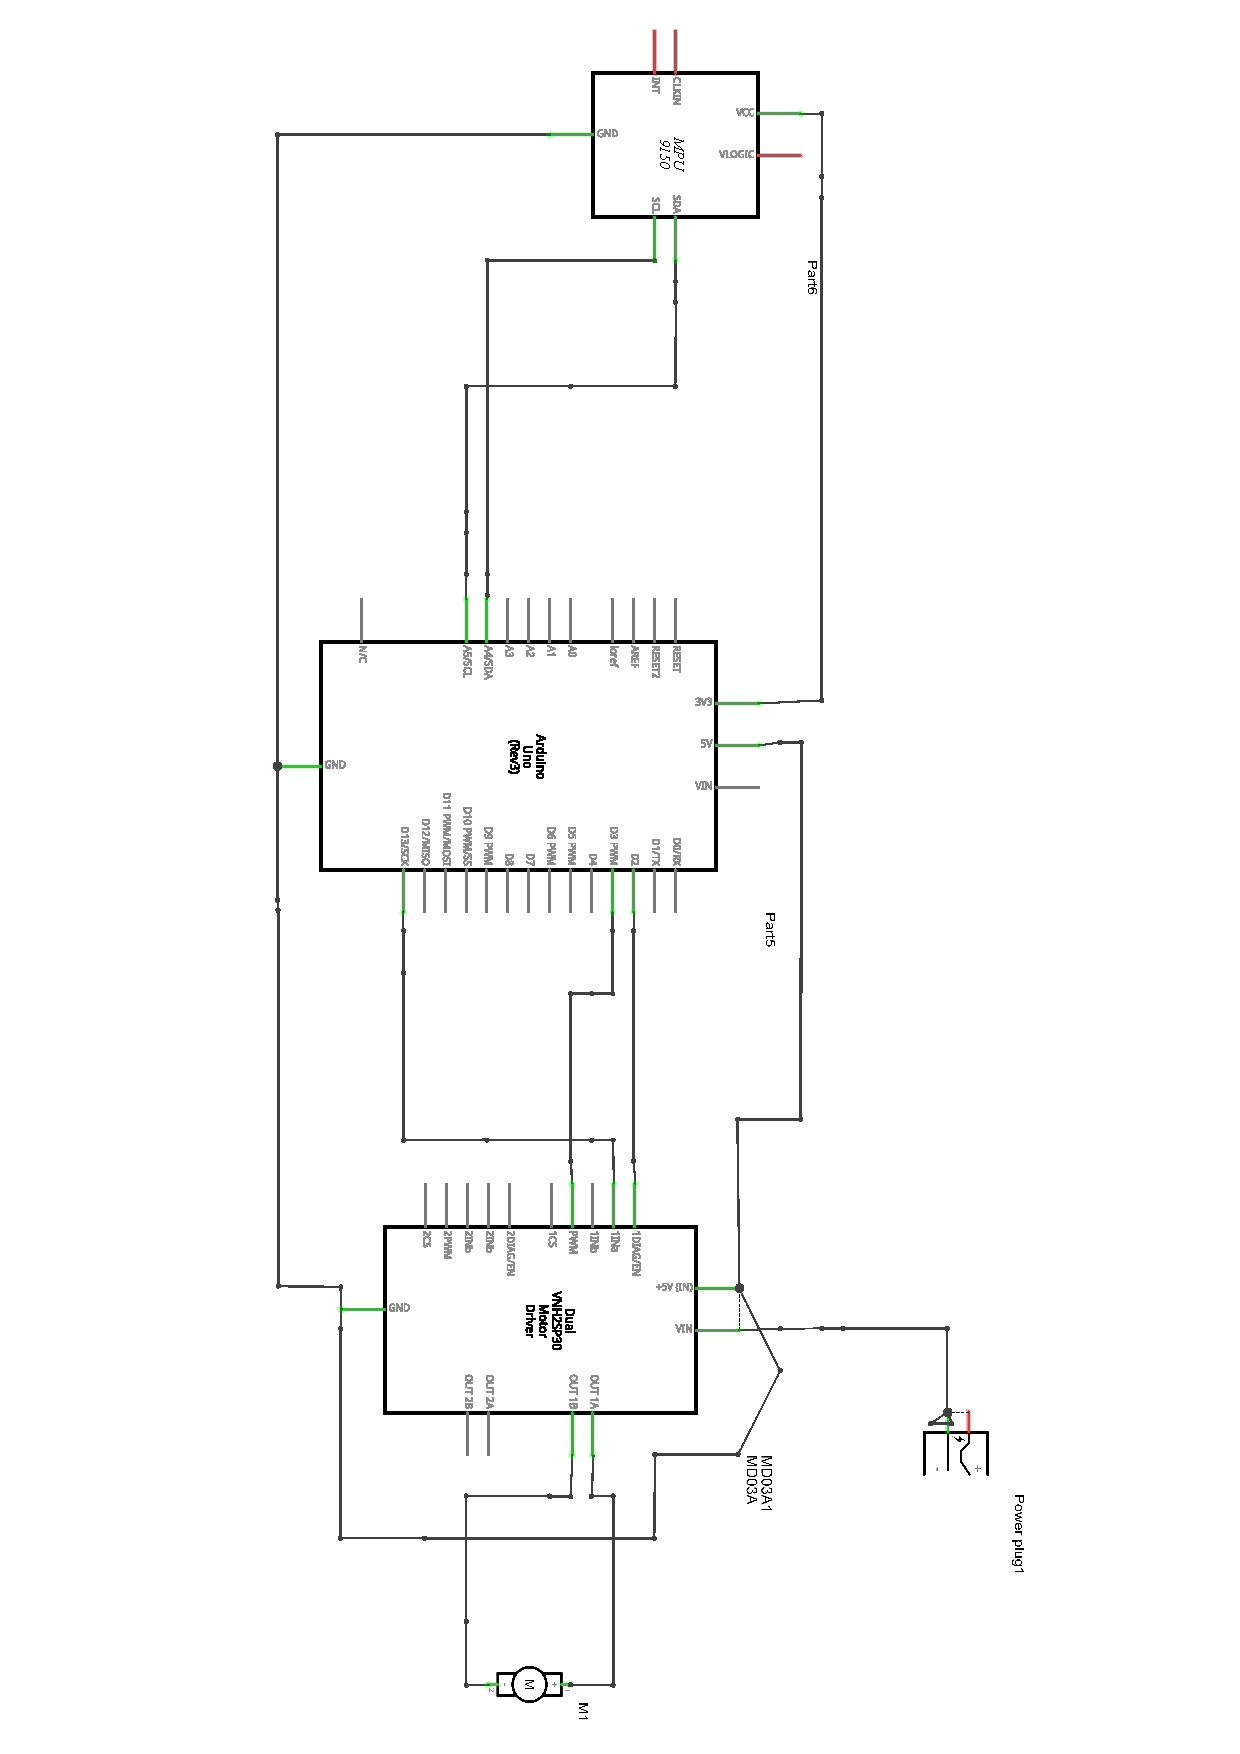
\includegraphics[scale=0.4]{total_schem.pdf}
\caption{Schematic of the electrical components}
\label{Fig: circuit}
\end{figure}


\cleardoublepage   
\cleartoverso %force back cover to be "left" page

\includepdf[pages={2}]{kth-cover.pdf}

%\printbibliography
\end{document}
